% Copyright © 2013 Martin Ueding <dev@martin-ueding.de>

% Copyright © 2012-2013 Martin Ueding <dev@martin-ueding.de>

% This is my general purpose LaTeX header file for writing German documents.
% Ideally, you include this using a simple ``% Copyright © 2012-2013 Martin Ueding <dev@martin-ueding.de>

% This is my general purpose LaTeX header file for writing German documents.
% Ideally, you include this using a simple ``% Copyright © 2012-2013 Martin Ueding <dev@martin-ueding.de>

% This is my general purpose LaTeX header file for writing German documents.
% Ideally, you include this using a simple ``\input{header.tex}`` in your main
% document and start with ``\title`` and ``\begin{document}`` afterwards.

% If you need to add additional packages, I recommend not doing this in this
% file, but in your main document. That way, you can just drop in a new
% ``header.tex`` and get all the new commands without having to merge manually.

% Since this file encorporates a CC-BY-SA fragment, this whole files is
% licensed under the CC-BY-SA license.

\documentclass[11pt, ngerman, fleqn, DIV=15, headinclude]{scrartcl}

\usepackage{graphicx}

% Environment to quote the problem. Currently, this is just a new name for the
% quote environment.
\newenvironment{problem}{\begin{quote}}{\end{quote}}

\usepackage{cleveref}

%%%%%%%%%%%%%%%%%%%%%%%%%%%%%%%%%%%%%%%%%%%%%%%%%%%%%%%%%%%%%%%%%%%%%%%%%%%%%%%
%                                Locale, date                                 %
%%%%%%%%%%%%%%%%%%%%%%%%%%%%%%%%%%%%%%%%%%%%%%%%%%%%%%%%%%%%%%%%%%%%%%%%%%%%%%%

\usepackage{babel}
\usepackage[iso]{isodate}

%%%%%%%%%%%%%%%%%%%%%%%%%%%%%%%%%%%%%%%%%%%%%%%%%%%%%%%%%%%%%%%%%%%%%%%%%%%%%%%
%                          Margins and other spacing                          %
%%%%%%%%%%%%%%%%%%%%%%%%%%%%%%%%%%%%%%%%%%%%%%%%%%%%%%%%%%%%%%%%%%%%%%%%%%%%%%%

\usepackage[parfill]{parskip}
\usepackage{setspace}
\usepackage[activate]{microtype}

\setlength{\columnsep}{2cm}

%%%%%%%%%%%%%%%%%%%%%%%%%%%%%%%%%%%%%%%%%%%%%%%%%%%%%%%%%%%%%%%%%%%%%%%%%%%%%%%
%                                    Color                                    %
%%%%%%%%%%%%%%%%%%%%%%%%%%%%%%%%%%%%%%%%%%%%%%%%%%%%%%%%%%%%%%%%%%%%%%%%%%%%%%%

\usepackage[usenames, dvipsnames]{xcolor}

\colorlet{darkred}{red!70!black}
\colorlet{darkblue}{blue!70!black}
\colorlet{darkgreen}{green!40!black}

%%%%%%%%%%%%%%%%%%%%%%%%%%%%%%%%%%%%%%%%%%%%%%%%%%%%%%%%%%%%%%%%%%%%%%%%%%%%%%%
%                         Font and font like settings                         %
%%%%%%%%%%%%%%%%%%%%%%%%%%%%%%%%%%%%%%%%%%%%%%%%%%%%%%%%%%%%%%%%%%%%%%%%%%%%%%%

% This replaces all fonts with Bitstream Charter, Bitstream Vera Sans and
% Bitstream Vera Mono. Math will be rendered in Charter.
\usepackage[charter, greekuppercase=italicized]{mathdesign}
\usepackage{beramono}
\usepackage{berasans}

% Bold, sans-serif tensors. This fragment is taken from “egreg” from
% http://tex.stackexchange.com/a/82747/8945 and licensed under `CC-BY-SA
% <https://creativecommons.org/licenses/by-sa/3.0/>`_.
\usepackage{bm}
\DeclareMathAlphabet{\mathsfit}{\encodingdefault}{\sfdefault}{m}{sl}
\SetMathAlphabet{\mathsfit}{bold}{\encodingdefault}{\sfdefault}{bx}{sl}
\newcommand{\tens}[1]{\bm{\mathsfit{#1}}}

% Bold vectors.
\renewcommand{\vec}[1]{\boldsymbol{#1}}

%%%%%%%%%%%%%%%%%%%%%%%%%%%%%%%%%%%%%%%%%%%%%%%%%%%%%%%%%%%%%%%%%%%%%%%%%%%%%%%
%                               Input encoding                                %
%%%%%%%%%%%%%%%%%%%%%%%%%%%%%%%%%%%%%%%%%%%%%%%%%%%%%%%%%%%%%%%%%%%%%%%%%%%%%%%

\usepackage[T1]{fontenc}
\usepackage[utf8]{inputenc}

%%%%%%%%%%%%%%%%%%%%%%%%%%%%%%%%%%%%%%%%%%%%%%%%%%%%%%%%%%%%%%%%%%%%%%%%%%%%%%%
%                         Hyperrefs and PDF metadata                          %
%%%%%%%%%%%%%%%%%%%%%%%%%%%%%%%%%%%%%%%%%%%%%%%%%%%%%%%%%%%%%%%%%%%%%%%%%%%%%%%

\usepackage{hyperref}
\usepackage{lastpage}

% This sets the author in the properties of the PDF as well. If you want to
% change it, just override it with another ``\hypersetup`` call.
\hypersetup{
	breaklinks=false,
	citecolor=darkgreen,
	colorlinks=true,
	linkcolor=darkblue,
	menucolor=black,
	pdfauthor={Martin Ueding},
	urlcolor=darkblue,
}

%%%%%%%%%%%%%%%%%%%%%%%%%%%%%%%%%%%%%%%%%%%%%%%%%%%%%%%%%%%%%%%%%%%%%%%%%%%%%%%
%                               Math Operators                                %
%%%%%%%%%%%%%%%%%%%%%%%%%%%%%%%%%%%%%%%%%%%%%%%%%%%%%%%%%%%%%%%%%%%%%%%%%%%%%%%

% AMS environments like ``align`` and theorems like ``proof``.
\usepackage{amsmath}
\usepackage{amsthm}

% Common math constructs like partial derivatives.
\usepackage{commath}

% Physical units.
\usepackage[output-decimal-marker={,}]{siunitx}

% Since I use mathdesign with italic uppercase greek characters, the Ohm unit will be displayed with an italic Ω by default. Units have to be roman, so this forces it the right way.
\DeclareSIUnit{\ohm}{$\Omegaup$}

% Word like operators.
\DeclareMathOperator{\acosh}{arcosh}
\DeclareMathOperator{\arcosh}{arcosh}
\DeclareMathOperator{\arcsinh}{arsinh}
\DeclareMathOperator{\arsinh}{arsinh}
\DeclareMathOperator{\asinh}{arsinh}
\DeclareMathOperator{\card}{card}
\DeclareMathOperator{\csch}{cshs}
\DeclareMathOperator{\diam}{diam}
\DeclareMathOperator{\sech}{sech}
\renewcommand{\Im}{\mathop{{}\mathrm{Im}}\nolimits}
\renewcommand{\Re}{\mathop{{}\mathrm{Re}}\nolimits}

% Fourier transform.
\DeclareMathOperator{\fourier}{\ensuremath{\mathcal{F}}}

% Roman versions of “e” and “i” to serve as Euler's number and the imaginary
% constant.
\newcommand{\ee}{\eup}
\newcommand{\eup}{\mathrm e}
\newcommand{\ii}{\iup}
\newcommand{\iup}{\mathrm i}

% Symbols for the various mathematical fields (natural numbers, integers,
% rational numbers, real numbers, complex numbers).
\newcommand{\C}{\ensuremath{\mathbb C}}
\newcommand{\N}{\ensuremath{\mathbb N}}
\newcommand{\Q}{\ensuremath{\mathbb Q}}
\newcommand{\R}{\ensuremath{\mathbb R}}
\newcommand{\Z}{\ensuremath{\mathbb Z}}

% Shape like operators.
\DeclareMathOperator{\dalambert}{\Box}
\DeclareMathOperator{\laplace}{\bigtriangleup}
\newcommand{\curl}{\vnabla \times}
\newcommand{\divergence}[1]{\inner{\vnabla}{#1}}
\newcommand{\vnabla}{\vec \nabla}

\newcommand{\half}{\frac 12}

% Unit vector (German „Einheitsvektor“).
\newcommand{\ev}{\hat{\vec e}}

% Scientific notation for large numbers.
\newcommand{\e}[1]{\cdot 10^{#1}}

% Mathematician's notation for the inner (scalar, dot) product.
\newcommand{\bracket}[1]{\left\langle #1 \right\rangle}
\newcommand{\inner}[2]{\bracket{#1, #2}}

% Placeholders.
\newcommand{\emesswert}{\del{\messwert \pm \messwert}}
\newcommand{\fehlt}{\textcolor{darkred}{Hier fehlen noch Inhalte.}}
\newcommand{\messwert}{\textcolor{blue}{\square}}
\newcommand{\punkte}{\phantom{xxxxx}}
\newcommand{\punktevon}[1]{\begin{flushright}/ #1\end{flushright}}

% Separator for equations on a single line.
\newcommand{\eqnsep}{,\quad}

% Quantum Mechanics
\usepackage{braket}

%%%%%%%%%%%%%%%%%%%%%%%%%%%%%%%%%%%%%%%%%%%%%%%%%%%%%%%%%%%%%%%%%%%%%%%%%%%%%%%
%                                  Headings                                   %
%%%%%%%%%%%%%%%%%%%%%%%%%%%%%%%%%%%%%%%%%%%%%%%%%%%%%%%%%%%%%%%%%%%%%%%%%%%%%%%

% This will set fancy headings to the top of the page. The page number will be
% accompanied by the total number of pages. That way, you will know if any page
% is missing.
%
% If you do not want this for your document, you can just use
% ``\pagestyle{plain}``.

\usepackage{scrpage2}

\pagestyle{scrheadings}
\automark{section}
\cfoot{\footnotesize{Seite \thepage\ / \pageref{LastPage}}}
\chead{}
\ihead{}
\ohead{\rightmark}
\setheadsepline{.4pt}

%%%%%%%%%%%%%%%%%%%%%%%%%%%%%%%%%%%%%%%%%%%%%%%%%%%%%%%%%%%%%%%%%%%%%%%%%%%%%%%
%                            Bibliography (BibTeX)                            %
%%%%%%%%%%%%%%%%%%%%%%%%%%%%%%%%%%%%%%%%%%%%%%%%%%%%%%%%%%%%%%%%%%%%%%%%%%%%%%%

\newcommand{\bibliographyfile}{../../zentrale_BibTeX/Central}
\bibliographystyle{apalike2}

%%%%%%%%%%%%%%%%%%%%%%%%%%%%%%%%%%%%%%%%%%%%%%%%%%%%%%%%%%%%%%%%%%%%%%%%%%%%%%%
%                                Abbreviations                                %
%%%%%%%%%%%%%%%%%%%%%%%%%%%%%%%%%%%%%%%%%%%%%%%%%%%%%%%%%%%%%%%%%%%%%%%%%%%%%%%

\newcommand{\dhabk}{\mbox{d.\,h.}}

%%%%%%%%%%%%%%%%%%%%%%%%%%%%%%%%%%%%%%%%%%%%%%%%%%%%%%%%%%%%%%%%%%%%%%%%%%%%%%%
%                                  Licences                                   %
%%%%%%%%%%%%%%%%%%%%%%%%%%%%%%%%%%%%%%%%%%%%%%%%%%%%%%%%%%%%%%%%%%%%%%%%%%%%%%%

\usepackage{ccicons}

\newcommand{\ccbysadetext}{%
	\begin{small}
		Dieses Werk bzw. Inhalt steht unter einer
		\href{http://creativecommons.org/licenses/by-sa/3.0/deed.de}{%
			Creative Commons Namensnennung - Weitergabe unter gleichen
		Bedingungen 3.0 Unported Lizenz}.
	\end{small}
}

\newcommand{\ccbysadetitle}{%
	Lizenz: \href{http://creativecommons.org/licenses/by-sa/3.0/deed.de}
	{CC-BY-SA 3.0 \ccbysa}
}
`` in your main
% document and start with ``\title`` and ``\begin{document}`` afterwards.

% If you need to add additional packages, I recommend not doing this in this
% file, but in your main document. That way, you can just drop in a new
% ``header.tex`` and get all the new commands without having to merge manually.

% Since this file encorporates a CC-BY-SA fragment, this whole files is
% licensed under the CC-BY-SA license.

\documentclass[11pt, ngerman, fleqn, DIV=15, headinclude]{scrartcl}

\usepackage{graphicx}

% Environment to quote the problem. Currently, this is just a new name for the
% quote environment.
\newenvironment{problem}{\begin{quote}}{\end{quote}}

\usepackage{cleveref}

%%%%%%%%%%%%%%%%%%%%%%%%%%%%%%%%%%%%%%%%%%%%%%%%%%%%%%%%%%%%%%%%%%%%%%%%%%%%%%%
%                                Locale, date                                 %
%%%%%%%%%%%%%%%%%%%%%%%%%%%%%%%%%%%%%%%%%%%%%%%%%%%%%%%%%%%%%%%%%%%%%%%%%%%%%%%

\usepackage{babel}
\usepackage[iso]{isodate}

%%%%%%%%%%%%%%%%%%%%%%%%%%%%%%%%%%%%%%%%%%%%%%%%%%%%%%%%%%%%%%%%%%%%%%%%%%%%%%%
%                          Margins and other spacing                          %
%%%%%%%%%%%%%%%%%%%%%%%%%%%%%%%%%%%%%%%%%%%%%%%%%%%%%%%%%%%%%%%%%%%%%%%%%%%%%%%

\usepackage[parfill]{parskip}
\usepackage{setspace}
\usepackage[activate]{microtype}

\setlength{\columnsep}{2cm}

%%%%%%%%%%%%%%%%%%%%%%%%%%%%%%%%%%%%%%%%%%%%%%%%%%%%%%%%%%%%%%%%%%%%%%%%%%%%%%%
%                                    Color                                    %
%%%%%%%%%%%%%%%%%%%%%%%%%%%%%%%%%%%%%%%%%%%%%%%%%%%%%%%%%%%%%%%%%%%%%%%%%%%%%%%

\usepackage[usenames, dvipsnames]{xcolor}

\colorlet{darkred}{red!70!black}
\colorlet{darkblue}{blue!70!black}
\colorlet{darkgreen}{green!40!black}

%%%%%%%%%%%%%%%%%%%%%%%%%%%%%%%%%%%%%%%%%%%%%%%%%%%%%%%%%%%%%%%%%%%%%%%%%%%%%%%
%                         Font and font like settings                         %
%%%%%%%%%%%%%%%%%%%%%%%%%%%%%%%%%%%%%%%%%%%%%%%%%%%%%%%%%%%%%%%%%%%%%%%%%%%%%%%

% This replaces all fonts with Bitstream Charter, Bitstream Vera Sans and
% Bitstream Vera Mono. Math will be rendered in Charter.
\usepackage[charter, greekuppercase=italicized]{mathdesign}
\usepackage{beramono}
\usepackage{berasans}

% Bold, sans-serif tensors. This fragment is taken from “egreg” from
% http://tex.stackexchange.com/a/82747/8945 and licensed under `CC-BY-SA
% <https://creativecommons.org/licenses/by-sa/3.0/>`_.
\usepackage{bm}
\DeclareMathAlphabet{\mathsfit}{\encodingdefault}{\sfdefault}{m}{sl}
\SetMathAlphabet{\mathsfit}{bold}{\encodingdefault}{\sfdefault}{bx}{sl}
\newcommand{\tens}[1]{\bm{\mathsfit{#1}}}

% Bold vectors.
\renewcommand{\vec}[1]{\boldsymbol{#1}}

%%%%%%%%%%%%%%%%%%%%%%%%%%%%%%%%%%%%%%%%%%%%%%%%%%%%%%%%%%%%%%%%%%%%%%%%%%%%%%%
%                               Input encoding                                %
%%%%%%%%%%%%%%%%%%%%%%%%%%%%%%%%%%%%%%%%%%%%%%%%%%%%%%%%%%%%%%%%%%%%%%%%%%%%%%%

\usepackage[T1]{fontenc}
\usepackage[utf8]{inputenc}

%%%%%%%%%%%%%%%%%%%%%%%%%%%%%%%%%%%%%%%%%%%%%%%%%%%%%%%%%%%%%%%%%%%%%%%%%%%%%%%
%                         Hyperrefs and PDF metadata                          %
%%%%%%%%%%%%%%%%%%%%%%%%%%%%%%%%%%%%%%%%%%%%%%%%%%%%%%%%%%%%%%%%%%%%%%%%%%%%%%%

\usepackage{hyperref}
\usepackage{lastpage}

% This sets the author in the properties of the PDF as well. If you want to
% change it, just override it with another ``\hypersetup`` call.
\hypersetup{
	breaklinks=false,
	citecolor=darkgreen,
	colorlinks=true,
	linkcolor=darkblue,
	menucolor=black,
	pdfauthor={Martin Ueding},
	urlcolor=darkblue,
}

%%%%%%%%%%%%%%%%%%%%%%%%%%%%%%%%%%%%%%%%%%%%%%%%%%%%%%%%%%%%%%%%%%%%%%%%%%%%%%%
%                               Math Operators                                %
%%%%%%%%%%%%%%%%%%%%%%%%%%%%%%%%%%%%%%%%%%%%%%%%%%%%%%%%%%%%%%%%%%%%%%%%%%%%%%%

% AMS environments like ``align`` and theorems like ``proof``.
\usepackage{amsmath}
\usepackage{amsthm}

% Common math constructs like partial derivatives.
\usepackage{commath}

% Physical units.
\usepackage[output-decimal-marker={,}]{siunitx}

% Since I use mathdesign with italic uppercase greek characters, the Ohm unit will be displayed with an italic Ω by default. Units have to be roman, so this forces it the right way.
\DeclareSIUnit{\ohm}{$\Omegaup$}

% Word like operators.
\DeclareMathOperator{\acosh}{arcosh}
\DeclareMathOperator{\arcosh}{arcosh}
\DeclareMathOperator{\arcsinh}{arsinh}
\DeclareMathOperator{\arsinh}{arsinh}
\DeclareMathOperator{\asinh}{arsinh}
\DeclareMathOperator{\card}{card}
\DeclareMathOperator{\csch}{cshs}
\DeclareMathOperator{\diam}{diam}
\DeclareMathOperator{\sech}{sech}
\renewcommand{\Im}{\mathop{{}\mathrm{Im}}\nolimits}
\renewcommand{\Re}{\mathop{{}\mathrm{Re}}\nolimits}

% Fourier transform.
\DeclareMathOperator{\fourier}{\ensuremath{\mathcal{F}}}

% Roman versions of “e” and “i” to serve as Euler's number and the imaginary
% constant.
\newcommand{\ee}{\eup}
\newcommand{\eup}{\mathrm e}
\newcommand{\ii}{\iup}
\newcommand{\iup}{\mathrm i}

% Symbols for the various mathematical fields (natural numbers, integers,
% rational numbers, real numbers, complex numbers).
\newcommand{\C}{\ensuremath{\mathbb C}}
\newcommand{\N}{\ensuremath{\mathbb N}}
\newcommand{\Q}{\ensuremath{\mathbb Q}}
\newcommand{\R}{\ensuremath{\mathbb R}}
\newcommand{\Z}{\ensuremath{\mathbb Z}}

% Shape like operators.
\DeclareMathOperator{\dalambert}{\Box}
\DeclareMathOperator{\laplace}{\bigtriangleup}
\newcommand{\curl}{\vnabla \times}
\newcommand{\divergence}[1]{\inner{\vnabla}{#1}}
\newcommand{\vnabla}{\vec \nabla}

\newcommand{\half}{\frac 12}

% Unit vector (German „Einheitsvektor“).
\newcommand{\ev}{\hat{\vec e}}

% Scientific notation for large numbers.
\newcommand{\e}[1]{\cdot 10^{#1}}

% Mathematician's notation for the inner (scalar, dot) product.
\newcommand{\bracket}[1]{\left\langle #1 \right\rangle}
\newcommand{\inner}[2]{\bracket{#1, #2}}

% Placeholders.
\newcommand{\emesswert}{\del{\messwert \pm \messwert}}
\newcommand{\fehlt}{\textcolor{darkred}{Hier fehlen noch Inhalte.}}
\newcommand{\messwert}{\textcolor{blue}{\square}}
\newcommand{\punkte}{\phantom{xxxxx}}
\newcommand{\punktevon}[1]{\begin{flushright}/ #1\end{flushright}}

% Separator for equations on a single line.
\newcommand{\eqnsep}{,\quad}

% Quantum Mechanics
\usepackage{braket}

%%%%%%%%%%%%%%%%%%%%%%%%%%%%%%%%%%%%%%%%%%%%%%%%%%%%%%%%%%%%%%%%%%%%%%%%%%%%%%%
%                                  Headings                                   %
%%%%%%%%%%%%%%%%%%%%%%%%%%%%%%%%%%%%%%%%%%%%%%%%%%%%%%%%%%%%%%%%%%%%%%%%%%%%%%%

% This will set fancy headings to the top of the page. The page number will be
% accompanied by the total number of pages. That way, you will know if any page
% is missing.
%
% If you do not want this for your document, you can just use
% ``\pagestyle{plain}``.

\usepackage{scrpage2}

\pagestyle{scrheadings}
\automark{section}
\cfoot{\footnotesize{Seite \thepage\ / \pageref{LastPage}}}
\chead{}
\ihead{}
\ohead{\rightmark}
\setheadsepline{.4pt}

%%%%%%%%%%%%%%%%%%%%%%%%%%%%%%%%%%%%%%%%%%%%%%%%%%%%%%%%%%%%%%%%%%%%%%%%%%%%%%%
%                            Bibliography (BibTeX)                            %
%%%%%%%%%%%%%%%%%%%%%%%%%%%%%%%%%%%%%%%%%%%%%%%%%%%%%%%%%%%%%%%%%%%%%%%%%%%%%%%

\newcommand{\bibliographyfile}{../../zentrale_BibTeX/Central}
\bibliographystyle{apalike2}

%%%%%%%%%%%%%%%%%%%%%%%%%%%%%%%%%%%%%%%%%%%%%%%%%%%%%%%%%%%%%%%%%%%%%%%%%%%%%%%
%                                Abbreviations                                %
%%%%%%%%%%%%%%%%%%%%%%%%%%%%%%%%%%%%%%%%%%%%%%%%%%%%%%%%%%%%%%%%%%%%%%%%%%%%%%%

\newcommand{\dhabk}{\mbox{d.\,h.}}

%%%%%%%%%%%%%%%%%%%%%%%%%%%%%%%%%%%%%%%%%%%%%%%%%%%%%%%%%%%%%%%%%%%%%%%%%%%%%%%
%                                  Licences                                   %
%%%%%%%%%%%%%%%%%%%%%%%%%%%%%%%%%%%%%%%%%%%%%%%%%%%%%%%%%%%%%%%%%%%%%%%%%%%%%%%

\usepackage{ccicons}

\newcommand{\ccbysadetext}{%
	\begin{small}
		Dieses Werk bzw. Inhalt steht unter einer
		\href{http://creativecommons.org/licenses/by-sa/3.0/deed.de}{%
			Creative Commons Namensnennung - Weitergabe unter gleichen
		Bedingungen 3.0 Unported Lizenz}.
	\end{small}
}

\newcommand{\ccbysadetitle}{%
	Lizenz: \href{http://creativecommons.org/licenses/by-sa/3.0/deed.de}
	{CC-BY-SA 3.0 \ccbysa}
}
`` in your main
% document and start with ``\title`` and ``\begin{document}`` afterwards.

% If you need to add additional packages, I recommend not doing this in this
% file, but in your main document. That way, you can just drop in a new
% ``header.tex`` and get all the new commands without having to merge manually.

% Since this file encorporates a CC-BY-SA fragment, this whole files is
% licensed under the CC-BY-SA license.

\documentclass[11pt, ngerman, fleqn, DIV=15, headinclude]{scrartcl}

\usepackage{graphicx}

% Environment to quote the problem. Currently, this is just a new name for the
% quote environment.
\newenvironment{problem}{\begin{quote}}{\end{quote}}

\usepackage{cleveref}

%%%%%%%%%%%%%%%%%%%%%%%%%%%%%%%%%%%%%%%%%%%%%%%%%%%%%%%%%%%%%%%%%%%%%%%%%%%%%%%
%                                Locale, date                                 %
%%%%%%%%%%%%%%%%%%%%%%%%%%%%%%%%%%%%%%%%%%%%%%%%%%%%%%%%%%%%%%%%%%%%%%%%%%%%%%%

\usepackage{babel}
\usepackage[iso]{isodate}

%%%%%%%%%%%%%%%%%%%%%%%%%%%%%%%%%%%%%%%%%%%%%%%%%%%%%%%%%%%%%%%%%%%%%%%%%%%%%%%
%                          Margins and other spacing                          %
%%%%%%%%%%%%%%%%%%%%%%%%%%%%%%%%%%%%%%%%%%%%%%%%%%%%%%%%%%%%%%%%%%%%%%%%%%%%%%%

\usepackage[parfill]{parskip}
\usepackage{setspace}
\usepackage[activate]{microtype}

\setlength{\columnsep}{2cm}

%%%%%%%%%%%%%%%%%%%%%%%%%%%%%%%%%%%%%%%%%%%%%%%%%%%%%%%%%%%%%%%%%%%%%%%%%%%%%%%
%                                    Color                                    %
%%%%%%%%%%%%%%%%%%%%%%%%%%%%%%%%%%%%%%%%%%%%%%%%%%%%%%%%%%%%%%%%%%%%%%%%%%%%%%%

\usepackage[usenames, dvipsnames]{xcolor}

\colorlet{darkred}{red!70!black}
\colorlet{darkblue}{blue!70!black}
\colorlet{darkgreen}{green!40!black}

%%%%%%%%%%%%%%%%%%%%%%%%%%%%%%%%%%%%%%%%%%%%%%%%%%%%%%%%%%%%%%%%%%%%%%%%%%%%%%%
%                         Font and font like settings                         %
%%%%%%%%%%%%%%%%%%%%%%%%%%%%%%%%%%%%%%%%%%%%%%%%%%%%%%%%%%%%%%%%%%%%%%%%%%%%%%%

% This replaces all fonts with Bitstream Charter, Bitstream Vera Sans and
% Bitstream Vera Mono. Math will be rendered in Charter.
\usepackage[charter, greekuppercase=italicized]{mathdesign}
\usepackage{beramono}
\usepackage{berasans}

% Bold, sans-serif tensors. This fragment is taken from “egreg” from
% http://tex.stackexchange.com/a/82747/8945 and licensed under `CC-BY-SA
% <https://creativecommons.org/licenses/by-sa/3.0/>`_.
\usepackage{bm}
\DeclareMathAlphabet{\mathsfit}{\encodingdefault}{\sfdefault}{m}{sl}
\SetMathAlphabet{\mathsfit}{bold}{\encodingdefault}{\sfdefault}{bx}{sl}
\newcommand{\tens}[1]{\bm{\mathsfit{#1}}}

% Bold vectors.
\renewcommand{\vec}[1]{\boldsymbol{#1}}

%%%%%%%%%%%%%%%%%%%%%%%%%%%%%%%%%%%%%%%%%%%%%%%%%%%%%%%%%%%%%%%%%%%%%%%%%%%%%%%
%                               Input encoding                                %
%%%%%%%%%%%%%%%%%%%%%%%%%%%%%%%%%%%%%%%%%%%%%%%%%%%%%%%%%%%%%%%%%%%%%%%%%%%%%%%

\usepackage[T1]{fontenc}
\usepackage[utf8]{inputenc}

%%%%%%%%%%%%%%%%%%%%%%%%%%%%%%%%%%%%%%%%%%%%%%%%%%%%%%%%%%%%%%%%%%%%%%%%%%%%%%%
%                         Hyperrefs and PDF metadata                          %
%%%%%%%%%%%%%%%%%%%%%%%%%%%%%%%%%%%%%%%%%%%%%%%%%%%%%%%%%%%%%%%%%%%%%%%%%%%%%%%

\usepackage{hyperref}
\usepackage{lastpage}

% This sets the author in the properties of the PDF as well. If you want to
% change it, just override it with another ``\hypersetup`` call.
\hypersetup{
	breaklinks=false,
	citecolor=darkgreen,
	colorlinks=true,
	linkcolor=darkblue,
	menucolor=black,
	pdfauthor={Martin Ueding},
	urlcolor=darkblue,
}

%%%%%%%%%%%%%%%%%%%%%%%%%%%%%%%%%%%%%%%%%%%%%%%%%%%%%%%%%%%%%%%%%%%%%%%%%%%%%%%
%                               Math Operators                                %
%%%%%%%%%%%%%%%%%%%%%%%%%%%%%%%%%%%%%%%%%%%%%%%%%%%%%%%%%%%%%%%%%%%%%%%%%%%%%%%

% AMS environments like ``align`` and theorems like ``proof``.
\usepackage{amsmath}
\usepackage{amsthm}

% Common math constructs like partial derivatives.
\usepackage{commath}

% Physical units.
\usepackage[output-decimal-marker={,}]{siunitx}

% Since I use mathdesign with italic uppercase greek characters, the Ohm unit will be displayed with an italic Ω by default. Units have to be roman, so this forces it the right way.
\DeclareSIUnit{\ohm}{$\Omegaup$}

% Word like operators.
\DeclareMathOperator{\acosh}{arcosh}
\DeclareMathOperator{\arcosh}{arcosh}
\DeclareMathOperator{\arcsinh}{arsinh}
\DeclareMathOperator{\arsinh}{arsinh}
\DeclareMathOperator{\asinh}{arsinh}
\DeclareMathOperator{\card}{card}
\DeclareMathOperator{\csch}{cshs}
\DeclareMathOperator{\diam}{diam}
\DeclareMathOperator{\sech}{sech}
\renewcommand{\Im}{\mathop{{}\mathrm{Im}}\nolimits}
\renewcommand{\Re}{\mathop{{}\mathrm{Re}}\nolimits}

% Fourier transform.
\DeclareMathOperator{\fourier}{\ensuremath{\mathcal{F}}}

% Roman versions of “e” and “i” to serve as Euler's number and the imaginary
% constant.
\newcommand{\ee}{\eup}
\newcommand{\eup}{\mathrm e}
\newcommand{\ii}{\iup}
\newcommand{\iup}{\mathrm i}

% Symbols for the various mathematical fields (natural numbers, integers,
% rational numbers, real numbers, complex numbers).
\newcommand{\C}{\ensuremath{\mathbb C}}
\newcommand{\N}{\ensuremath{\mathbb N}}
\newcommand{\Q}{\ensuremath{\mathbb Q}}
\newcommand{\R}{\ensuremath{\mathbb R}}
\newcommand{\Z}{\ensuremath{\mathbb Z}}

% Shape like operators.
\DeclareMathOperator{\dalambert}{\Box}
\DeclareMathOperator{\laplace}{\bigtriangleup}
\newcommand{\curl}{\vnabla \times}
\newcommand{\divergence}[1]{\inner{\vnabla}{#1}}
\newcommand{\vnabla}{\vec \nabla}

\newcommand{\half}{\frac 12}

% Unit vector (German „Einheitsvektor“).
\newcommand{\ev}{\hat{\vec e}}

% Scientific notation for large numbers.
\newcommand{\e}[1]{\cdot 10^{#1}}

% Mathematician's notation for the inner (scalar, dot) product.
\newcommand{\bracket}[1]{\left\langle #1 \right\rangle}
\newcommand{\inner}[2]{\bracket{#1, #2}}

% Placeholders.
\newcommand{\emesswert}{\del{\messwert \pm \messwert}}
\newcommand{\fehlt}{\textcolor{darkred}{Hier fehlen noch Inhalte.}}
\newcommand{\messwert}{\textcolor{blue}{\square}}
\newcommand{\punkte}{\phantom{xxxxx}}
\newcommand{\punktevon}[1]{\begin{flushright}/ #1\end{flushright}}

% Separator for equations on a single line.
\newcommand{\eqnsep}{,\quad}

% Quantum Mechanics
\usepackage{braket}

%%%%%%%%%%%%%%%%%%%%%%%%%%%%%%%%%%%%%%%%%%%%%%%%%%%%%%%%%%%%%%%%%%%%%%%%%%%%%%%
%                                  Headings                                   %
%%%%%%%%%%%%%%%%%%%%%%%%%%%%%%%%%%%%%%%%%%%%%%%%%%%%%%%%%%%%%%%%%%%%%%%%%%%%%%%

% This will set fancy headings to the top of the page. The page number will be
% accompanied by the total number of pages. That way, you will know if any page
% is missing.
%
% If you do not want this for your document, you can just use
% ``\pagestyle{plain}``.

\usepackage{scrpage2}

\pagestyle{scrheadings}
\automark{section}
\cfoot{\footnotesize{Seite \thepage\ / \pageref{LastPage}}}
\chead{}
\ihead{}
\ohead{\rightmark}
\setheadsepline{.4pt}

%%%%%%%%%%%%%%%%%%%%%%%%%%%%%%%%%%%%%%%%%%%%%%%%%%%%%%%%%%%%%%%%%%%%%%%%%%%%%%%
%                            Bibliography (BibTeX)                            %
%%%%%%%%%%%%%%%%%%%%%%%%%%%%%%%%%%%%%%%%%%%%%%%%%%%%%%%%%%%%%%%%%%%%%%%%%%%%%%%

\newcommand{\bibliographyfile}{../../zentrale_BibTeX/Central}
\bibliographystyle{apalike2}

%%%%%%%%%%%%%%%%%%%%%%%%%%%%%%%%%%%%%%%%%%%%%%%%%%%%%%%%%%%%%%%%%%%%%%%%%%%%%%%
%                                Abbreviations                                %
%%%%%%%%%%%%%%%%%%%%%%%%%%%%%%%%%%%%%%%%%%%%%%%%%%%%%%%%%%%%%%%%%%%%%%%%%%%%%%%

\newcommand{\dhabk}{\mbox{d.\,h.}}

%%%%%%%%%%%%%%%%%%%%%%%%%%%%%%%%%%%%%%%%%%%%%%%%%%%%%%%%%%%%%%%%%%%%%%%%%%%%%%%
%                                  Licences                                   %
%%%%%%%%%%%%%%%%%%%%%%%%%%%%%%%%%%%%%%%%%%%%%%%%%%%%%%%%%%%%%%%%%%%%%%%%%%%%%%%

\usepackage{ccicons}

\newcommand{\ccbysadetext}{%
	\begin{small}
		Dieses Werk bzw. Inhalt steht unter einer
		\href{http://creativecommons.org/licenses/by-sa/3.0/deed.de}{%
			Creative Commons Namensnennung - Weitergabe unter gleichen
		Bedingungen 3.0 Unported Lizenz}.
	\end{small}
}

\newcommand{\ccbysadetitle}{%
	Lizenz: \href{http://creativecommons.org/licenses/by-sa/3.0/deed.de}
	{CC-BY-SA 3.0 \ccbysa}
}


\usepackage{placeins}

\ihead{physik313 – Versuch 1}
\ifoot{Ueding, Lemmer}

\hypersetup{
	pdftitle={Ausbreitung von Signalen auf Leitungen}
}

\subject{Praktikumsprotokoll}
\title{Ausbreitung von Signalen auf Leitungen}
\subtitle{physik313 – Versuch 1}
\author{
	Martin Ueding \footnote{\href{mailto:mu@martin-ueding.de}{mu@martin-ueding.de}}
	\and
	Lino Lemmer \footnote{\href{mailto:s6lilemm@uni-bonn.de}{s6lilemm@uni-bonn.de}}
}
\publishers{Gruppe 3 -- A -- Brezina}

\setcounter{tocdepth}{2}

\begin{document}

\maketitle

Der \LaTeX{} Quelltext zu diesem Protokoll kann auf \url{http://martin-ueding.de/de/university/physik313/} eingesehen werden.

%\newpage
\tableofcontents
\newpage

%%%%%%%%%%%%%%%%%%%%%%%%%%%%%%%%%%%%%%%%%%%%%%%%%%%%%%%%%%%%%%%%%%%%%%%%%%%%%%%
%                                 Einleitung                                  %
%%%%%%%%%%%%%%%%%%%%%%%%%%%%%%%%%%%%%%%%%%%%%%%%%%%%%%%%%%%%%%%%%%%%%%%%%%%%%%%

\section{Einleitung}

In diesem Versuch experimentieren wir mit der Ausbreitung von Pulsen auf
Koaxialkabeln. Dabei betrachten wir Verzögerung, Reflexion und
Impulsdeformation.

%%%%%%%%%%%%%%%%%%%%%%%%%%%%%%%%%%%%%%%%%%%%%%%%%%%%%%%%%%%%%%%%%%%%%%%%%%%%%%%
%                                   Theorie                                   %
%%%%%%%%%%%%%%%%%%%%%%%%%%%%%%%%%%%%%%%%%%%%%%%%%%%%%%%%%%%%%%%%%%%%%%%%%%%%%%%

\newcommand\Uh{U_\text h}
\newcommand\Ur{U_\text r}

\section{Theorie}

In diesem Versuch werden die BNC-Kabel eingeführt. Diese bestehen aus einem
Leiter in der Mitte und einer geerdeten Abschrimung in einem großeren Radius.
Die beiden Leiter sind konzentrisch.

Widerstand $R$, Induktivität $L$, Verlustleitwert $G$ und Kapazität $C$ sind
alle proportional zur Kabellänge, so dass die Leitungskonstanten eingeführt
werden. Diese sind $R' = R/l$ und analog für die Anderen.

\subsection{Wellengleichung}

Eine vereinfachte Herleitung zerlegt das lange Kabel in viele $LC$-Glieder. Für
jedes differentielle Glied sind die Leitungskonstanten entscheidend. Aus den
Strom- und Spannungsgleichungen an den vier Polen kann eine Wellengleichung
hergeleitet werden. Dazu beginnt man mit:
\[
	U(x) = I(x) \Deltaup Z + U(x + \Deltaup x)
	\eqnsep
	I(x) = I(x + \Deltaup x) + U(x + \Deltaup x) \Deltaup Y
\]

Es folgen einige Umformungsschritte, Teilen durch $\Deltaup x$ und der
Grenzübergang $\Deltaup x \to 0$. Es entstehen zwei Differentialgleichungen,
die ineinander eingesetzt werden können und die Wellengleichung ergibt:
\[
	\dod[2] Ux = \Upsilon^2 U = 0
\]

Das $\Upsilon$ ist wie folgt definiert:
\begin{equation}
	\label{eq:1.6}
	\Upsilon^2 = Z' Y'
\end{equation}

Lösungen dieser Differentialgleichung sind ebene Wellen:
\begin{equation}
	\label{eq:1.7}
	\Uh(l) + \Ur(l)
	= \del{\Uh(0) \eup^{-\Upsilon x} + \Ur(0) \eup^{\Upsilon x}} \eup^{\iup \omega t}
\end{equation}

\subsection{Phasengeschwindigkeit}

Die Phasengeschwindigkeit kann hergeleitet werden zu:
\begin{equation}
	\label{eq:1.13}
	v_\text{ph} = c_0 \frac{1}{\sqrt{\varepsilon_0 \mu_0}}
\end{equation}

Der Wellenwiderstand ist in der Anleitung definiert als:
\begin{equation}
	\label{eq:1.14}
	Z = \frac{\Uh (x)}{I_\text h (x)}
\end{equation}

\subsection{Anpassung}

Die zurücklaufende Welle ist in der Regel nicht erwünscht und sollte am Ende
absorbiert werden. Die nennt man \emph{Anpassung}. Durch einen Widerstand am
Ende, der genauso groß wie der Wellenwiderstand des Kabels ist, kann die Welle
komplett absorbiert werden. Für den Funktionsgenerator sieht das Kabel dann
aus, wie ein unendlich langes, von dem keine Reflexion zu erwarten ist. 

Der richtige Abschlusswiderstand ist durch folgende Relation gegeben:
\begin{equation}
	\label{eq:1.17}
	R_\text A
	= \frac{\Uh (l) + \Ur (l)}{I_\text h (l) + I_\text r (l)}
	= Z \frac{U_{\text h l} + U_{\text r l}}{U_{\text h l} + I_{\text r l}}
	= Z \frac{1+r}{1-r}
\end{equation}

Dabei können drei Spezialfälle unterschieden werden, der angepasste Abschluss,
die offene Leitung und der Kurzschluss. Wie bei einer normalen Welle, die an
einem losen oder festen Ende reflektiert wird, nimmt der Reflexionsfaktor den
Wert \num{+1} bzw. \num{-1} an.

%%%%%%%%%%%%%%%%%%%%%%%%%%%%%%%%%%%%%%%%%%%%%%%%%%%%%%%%%%%%%%%%%%%%%%%%%%%%%%%
%                                  Aufgaben                                   %
%%%%%%%%%%%%%%%%%%%%%%%%%%%%%%%%%%%%%%%%%%%%%%%%%%%%%%%%%%%%%%%%%%%%%%%%%%%%%%%

\section{Aufgaben}

\subsection{Aufgabe A}

\begin{problem}
	Was muss man tun, um große Verzögerungszeiten zu erreichen?
\end{problem}

Eine große Verzögerungszeit bedeutet eine kleine Phasengeschwindigkeit. Diese
ist in Formel \eqref{eq:1.13} gegeben. Es kann entweder $\mu_r$ oder
$\varepsilon_r$ groß gemacht werden.

Außerdem kann das Kabel verlängert werden, dann braucht das Signal auch länger.

\subsection{Aufgabe B}

\begin{problem}
	Welche Konsequenz für den Wellenwiderstand haben die verschiedenen
	Möglichkeiten, die Verzögerungszeiten zu verändern?
\end{problem}

\paragraph{Permittivität erhöhen}

Durch Einfügen eines Dielektrikums kann die Permittivität erhöht werden,
dadurch werden die Kabel schwerer und teurer. Nach \eqref{eq:1.15} sinkt die
Impedanz $Z$ des Kabels mit größer werdender Permittivität.

\paragraph{Permeabilität erhöhen}

Durch Erhöhen der Permeabilität wird ebenfalls mehr Material gebraucht. Die
Impedanz steigt nach \eqref{eq:1.15} jetzt allerdings an.

Durch eine geschickte Kombination von Permittivität und Permeabilität kann die
Impedanz gleich gehalten werden und die Phasengeschwindigkeit verringert
werden.

\paragraph{Kabel verlängern}

Ein längeres Kabel bedeutet auch erhöhte normale Ohm'sche Verluste. Es braucht
auch mehr Material und somit mehr Gewicht und Kosten.

\subsection{Aufgabe C}

\begin{problem}
	Sei ein Kabel abgeschlossen mit $R_A = Z$. Wie hängt der Eingangswiderstand
	$R_\text{in}$ des Kabels von seiner Länge ab?
\end{problem}

Der Eingangswiderstand ist der Widerstand, den der Signalgenerator am Kabel
erfährt, also das Verhältnis von $\Uh(0)$ und $I_\text h(0)$. Der
Wellenwiderstand $Z$ ist ebenfalls dieses Verhältnis, wenn es keine
zurücklaufende Welle gibt, siehe \eqref{eq:1.14}.

Bei einer Länge $l$ hat es die spezifische Impedanz von $Z' = Z/l$. Die
Impedanz bei einer Länge $l$ ist somit $Z(l) = Z' l$. Für die
Längenabhängigkeit erhalten wir also:
\[
	R_\text{in}(l) = Z' l = Z
\]

\subsection{Aufgabe D}

\begin{problem}
	Wie groß ist die Eingangsimpedanz $Z$ eines verlustfreien Kabels mit
	Wellenwiderstand $Z = \SI{50}\ohm$ und einem offenen Leitungsende für eine
	Sinusspannung der Frequenz $\omega$ und der Wellenlänge auf dem Kabel
	$\lambda$ in Abhängigkeit der Länge $l$ des Kabels ($0 < l < \lambda$)?
\end{problem}

Nach \eqref{eq:1.14} ist der Wellenwiderstand:
\begin{equation}
	\label{eq:D1}
	Z := \frac{\Uh(x)}{I_\text h(x)}
\end{equation}

Wäre nicht die rücklaufende Welle, wäre hier einfach $Z_\text{in} = Z$. In
dieser Aufgabe habe ich zwar schon $Z$, allerdings reicht das nicht aus. Ich
brauche:
\begin{equation}
	\label{eq:D2}
	Z_\text{in}
	= \frac{\Uh (l) + \Ur (l)}{I_\text h (l) + I_\text r (l)}
\end{equation}

In der Anleitung steht für die offene Leitung
\[
	I_\text r(l) + I_\text h(l) = 0
\]
sowie
\[
	\Ur(l) - \Uh(l) = 0.
\]

Mit \eqref{eq:1.7} können wir herleiten:
\begin{align*}
	\Ur(l) &= \Uh(l) \\
	\Uh(0) \eup^{-\Upsilon x} \eup^{\iup \omega t} &= \Ur(0) \eup^{\Upsilon x}) \eup^{\iup \omega t} \\
	\Uh(0) \eup^{-\Upsilon x} &= \Ur(0) \eup^{\Upsilon x}) \\
	\Uh(0) \eup^{-2 \Upsilon x} &= \Ur(0) \\
\end{align*}

Für den Strom geht dies analog und führt auf die gleiche Phase zwischen ein-
und ausgehender Welle. Damit können wir \eqref{eq:D2} umschreiben und erhalten:
\[
	Z_\text{in}
	= \frac{\Uh (l)}{I_\text h (l)} (1 + \eup^{-2 \Upsilon x}
\]

In diese Relation setzen wir wiederum \eqref{eq:D1} ein und vereinfachen so zu:
\[
	Z_\text{in}
	= Z (1 + \eup^{-2 \Upsilon x}
\]

Das Kabel war als verlustfrei vorgegeben, es gibt also keinen Strom zwischen
Leiter und Masse. Damit ist $Y = Y' = 0$ Aus \eqref{eq:1.6} folgt damit, dass
$\Upsilon = 0$ ist. Dadurch ist der Phasenfaktor in der obigen Formel einfach
eins.

Wir erhalten das Ergebnis:
\[
	Z_\text{in} = 2 Z
\]

Dies ist unabhängig von der Länge und der Wellenlänge sowie der Frequenz.

%%%%%%%%%%%%%%%%%%%%%%%%%%%%%%%%%%%%%%%%%%%%%%%%%%%%%%%%%%%%%%%%%%%%%%%%%%%%%%%
%                      Versuchsaufbau und -durchführung                      %
%%%%%%%%%%%%%%%%%%%%%%%%%%%%%%%%%%%%%%%%%%%%%%%%%%%%%%%%%%%%%%%%%%%%%%%%%%%%%%%

\section{Versuchsaufbau und -durchführung}

\subsection{Seriennummern}

Die Seriennummern unserer Geräte haben wir in Tabelle \ref{tb:seriennummern}
aufgelistet.

\begin{table}[hb]
	\center
	\caption{Seriennummern unserer Geräte}
	\label{tb:seriennummern}
	\begin{tabular}{ll}
		Gerät & Seriennummer \\
		\hline
		Oszillograph & HM 604, 11/92, Z 20462 \\
		Funktionsgenerator & 3478 \\
		%Kabel HH 2500 & \\
		%Kabelkasten (RG-58 C/U) & \\
		%Differenzierglied & \\
		%Differenzierglied mit \SI{2.2}{\kilo\ohm} Anpassung & \\
		%Anpasswiderstand: \SI{2.45}{\kilo\ohm} & \\
		%Abschlusswiderstand: \SI{2.5}{\kilo\ohm} und \SI{50}{\ohm} & \\
		%Einstellbarer Abschlusswiderstand: \SIrange{0}{10}{\kilo\ohm} &
	\end{tabular}
\end{table}

\subsection{Versuchsaufgabe 1: Differenzierglied}

Wir schließen den Oszillograph an das Differenzierglied ohne Abschluss), das
vom Funktionsgenerator mit einer Rechteckspannung versorgt wird. Das
Oszillogramm ist in Abbildung \ref{fig:0752} dargestellt. Mit dem eingebauten
\SI{2.2}{\kilo\ohm} Widerstand werden die Impulse deutlich kleiner, wie in
Abbildung \ref{fig:0753} zu sehen.

\begin{figure}
	\centering
	\begin{minipage}{.45\linewidth}
	\end{minipage}
	\hfill
	\begin{minipage}{.45\linewidth}
	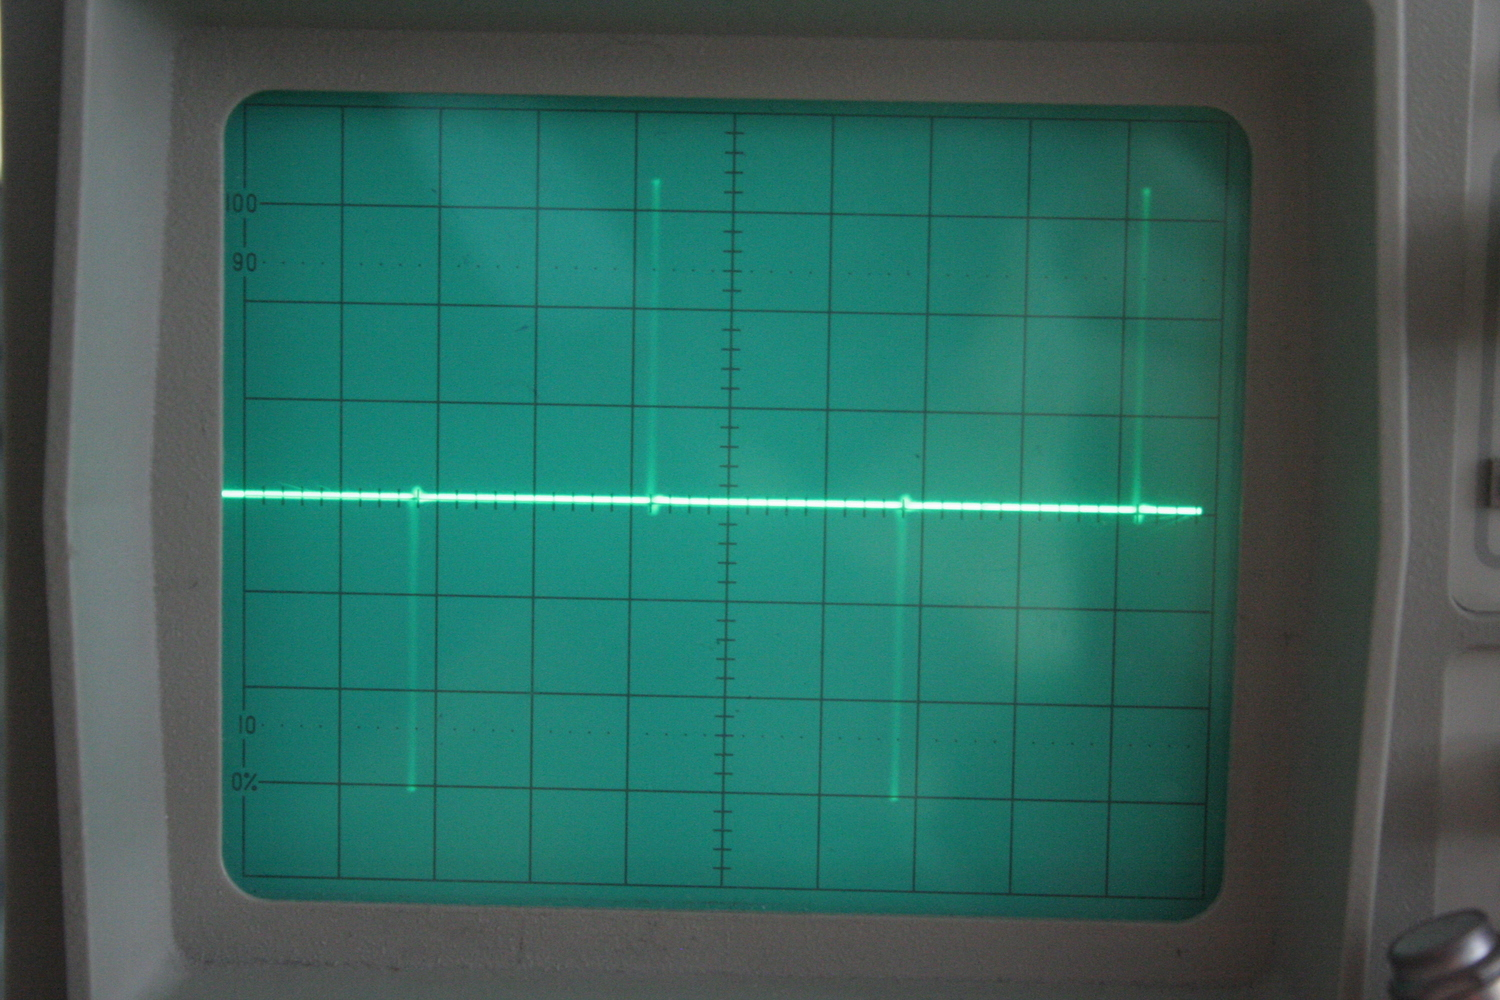
\includegraphics[width=\linewidth]{Fotos/IMG_0752-1500.jpg}
	\end{minipage}
	\caption{%
		Rechteck, Frequenz \SI{200}{\kilo\hertz}, Zeitbasis \SI{1}{\micro\second\per\division}, Verstärkung \SI{5}{\milli\volt\per\division}, externe Triggerung
	}
	\label{fig:0752}
\end{figure}

\begin{figure}
	\centering
	\begin{minipage}{.45\linewidth}
	\end{minipage}
	\hfill
	\begin{minipage}{.45\linewidth}
	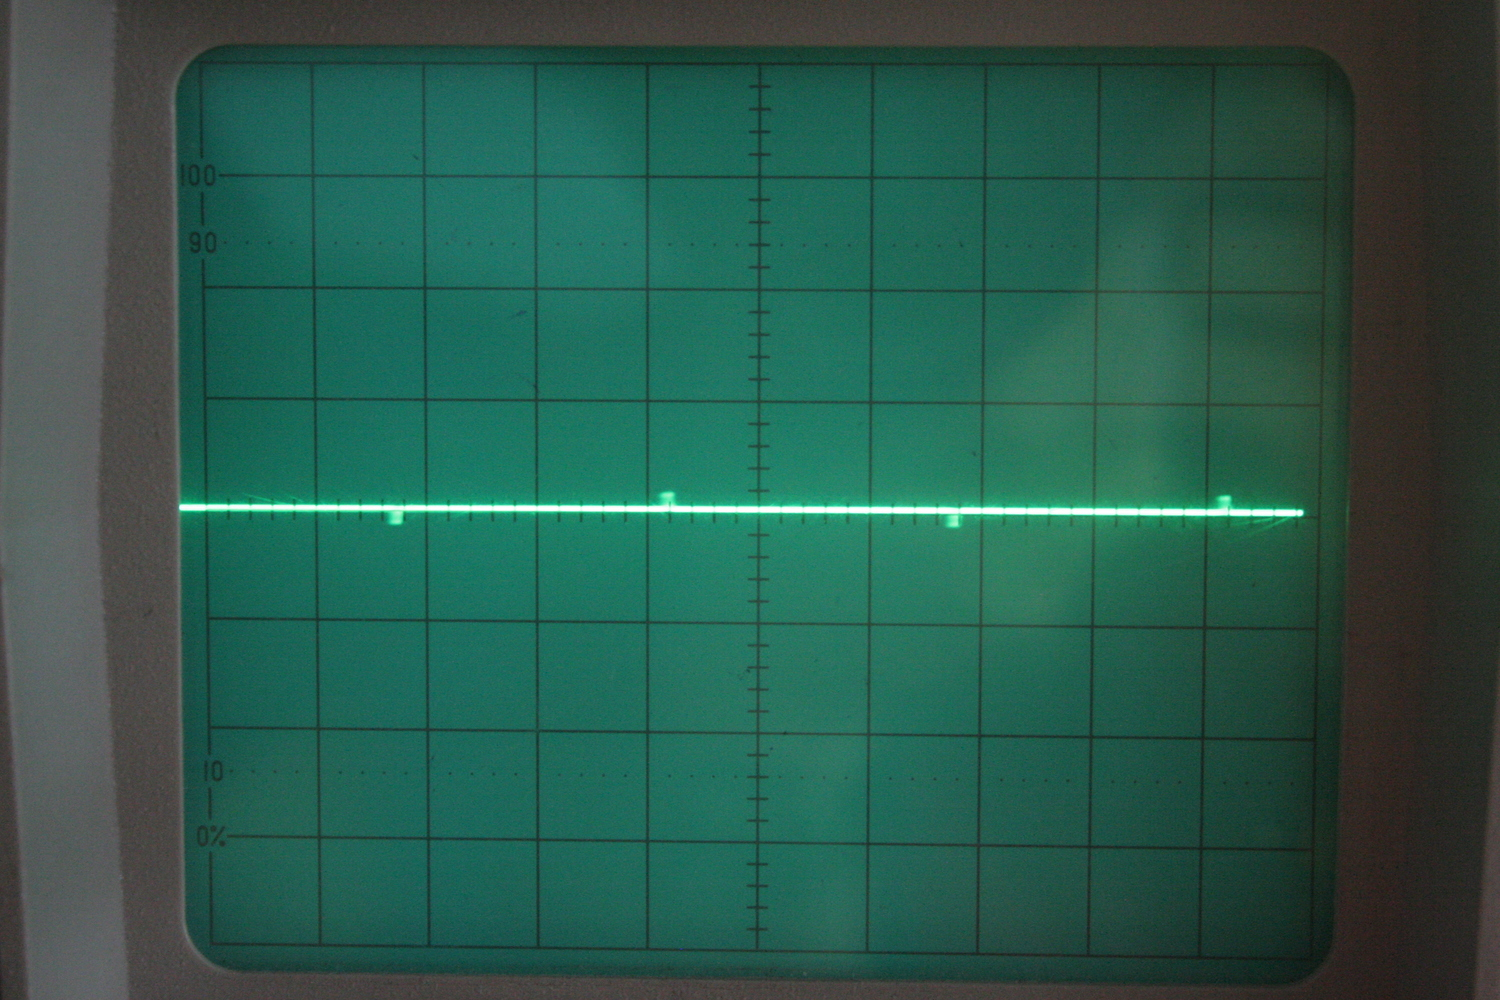
\includegraphics[width=\linewidth]{Fotos/IMG_0753-1500.jpg}
	\end{minipage}
	\caption{%
		Rechteck, Frequenz \SI{200}{\kilo\hertz}, Zeitbasis \SI{1}{\micro\second\per\division}, Verstärkung \SI{5}{\milli\volt\per\division}, externe Triggerung
	}
	\label{fig:0753}
\end{figure}

Durch den zusätzlichen Widerstand wird das Signal gedämpft. Außerdem kommt es zur Reflexion am offenen Ende, da der Anpasswiderstand im Differenzierglied durch den zusätzlichen Widerstand aufgehoben wird.

Ohne einen Abschlusswiderstand T-Stück am Oszilloskop sind die Peaks weniger deutlich ausgeprägt, siehe Abbildung \ref{fig:0755}.

\begin{figure}
	\centering
	\begin{minipage}{.45\linewidth}
	\end{minipage}
	\hfill
	\begin{minipage}{.45\linewidth}
	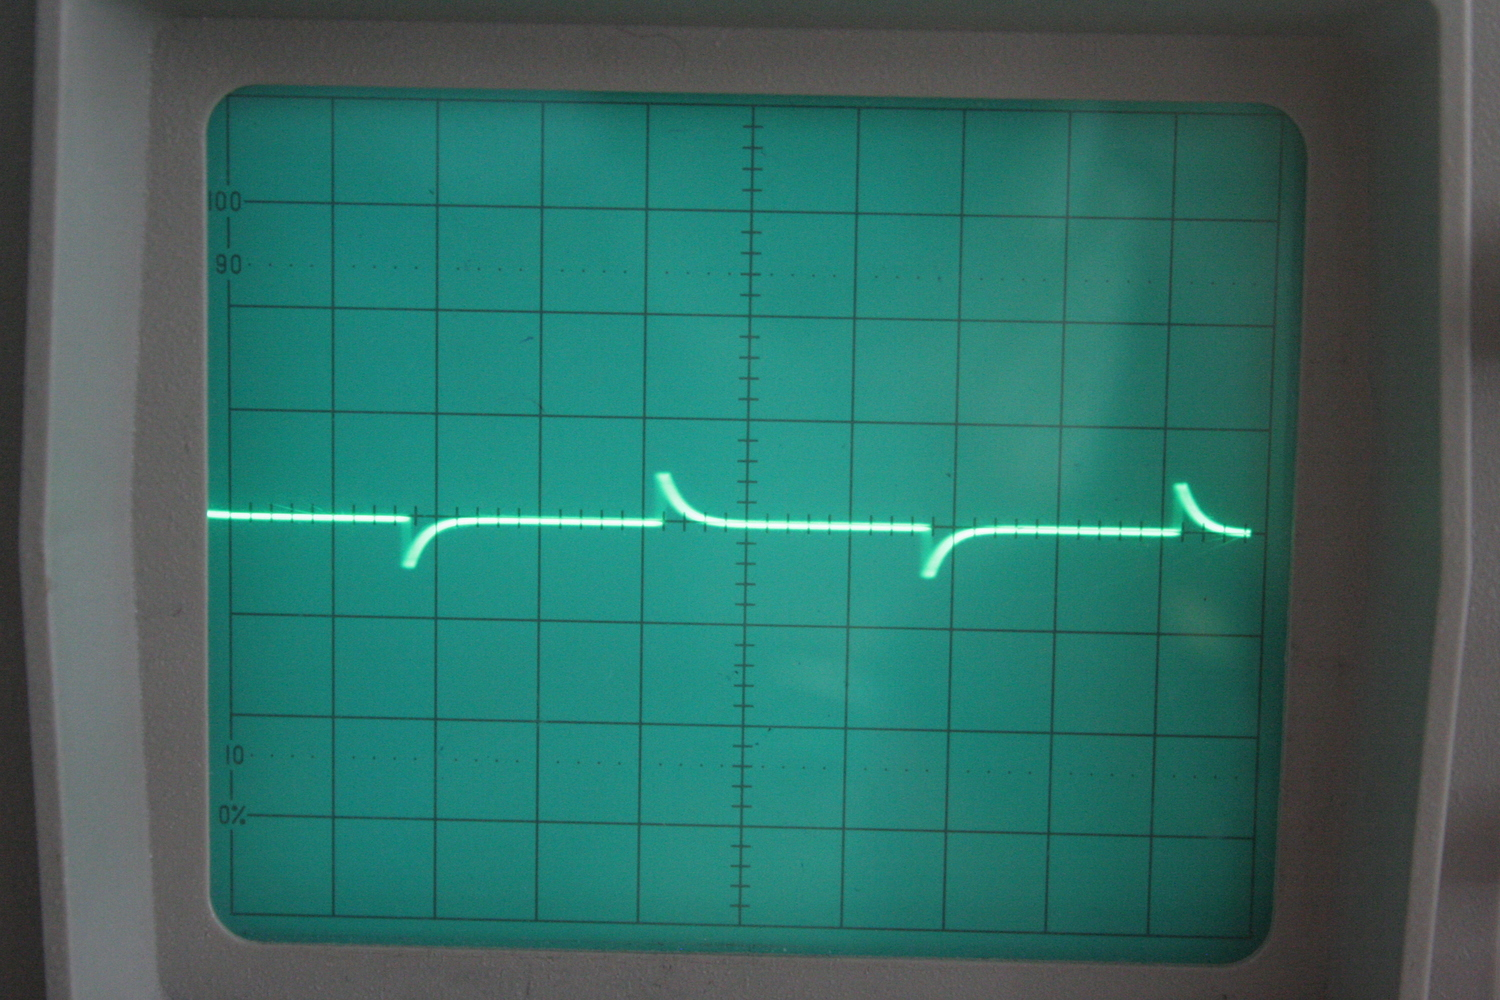
\includegraphics[width=\linewidth]{Fotos/IMG_0755-1500.jpg}
	\end{minipage}
	\caption{%
		Rechteck, Frequenz \SI{200}{\kilo\hertz}, Zeitbasis \SI{1}{\micro\second\per\division}, Verstärkung \SI{20}{\milli\volt\per\division}, externe Triggerung
	}
	\label{fig:0755}
\end{figure}

Die Zeit $\Deltaup t$ wird länger, $V_\text{SS}$ nimmt um einen Faktor 5 ab.

\FloatBarrier
\subsection{Versuchsaufgabe 2: Impulse auf Kabeln}

In diesem Versuchsteil schließen wir das Differenzierglied mit Zusatzwiderstand
an den Kanal 1 des Oszilloskops an. An den Kanal 2 schließen wir die Mitte der
beiden \SI{6}{\meter} Kabel an, so dass wir die Schwingung innerhalb des Kabels
beobachten können. Durch den Abschlusswiderstand im Differenzierglied und den
fehlenden Abschlusswiderstand am anderen Ende des Verzögerungskabels gehen die
Wellen im langen Kabel hin uns her und werden reflektiert.

Wir beobachten Wellenpakete (Abbildung \ref{fig:0756} und \ref{fig:0757}), die
oberhalb und unterhalb der Nulllinie sind. Um das Paket ist eine abfallende
Einhüllende, es sieht exponentiell aus. Auf Kanal 2 ist das Signal schwächer.
Da der Differenzierer abwechselnd positive und negative Peaks erzeugt, sind die
Wellenpakete auch abwechselnd über und unter der Nulllinie. Die Reflexion an
den beiden Enden kehrt die Amplitude nicht um.

\begin{figure}
	\centering
	\begin{minipage}{.45\linewidth}
	\end{minipage}
	\hfill
	\begin{minipage}{.45\linewidth}
	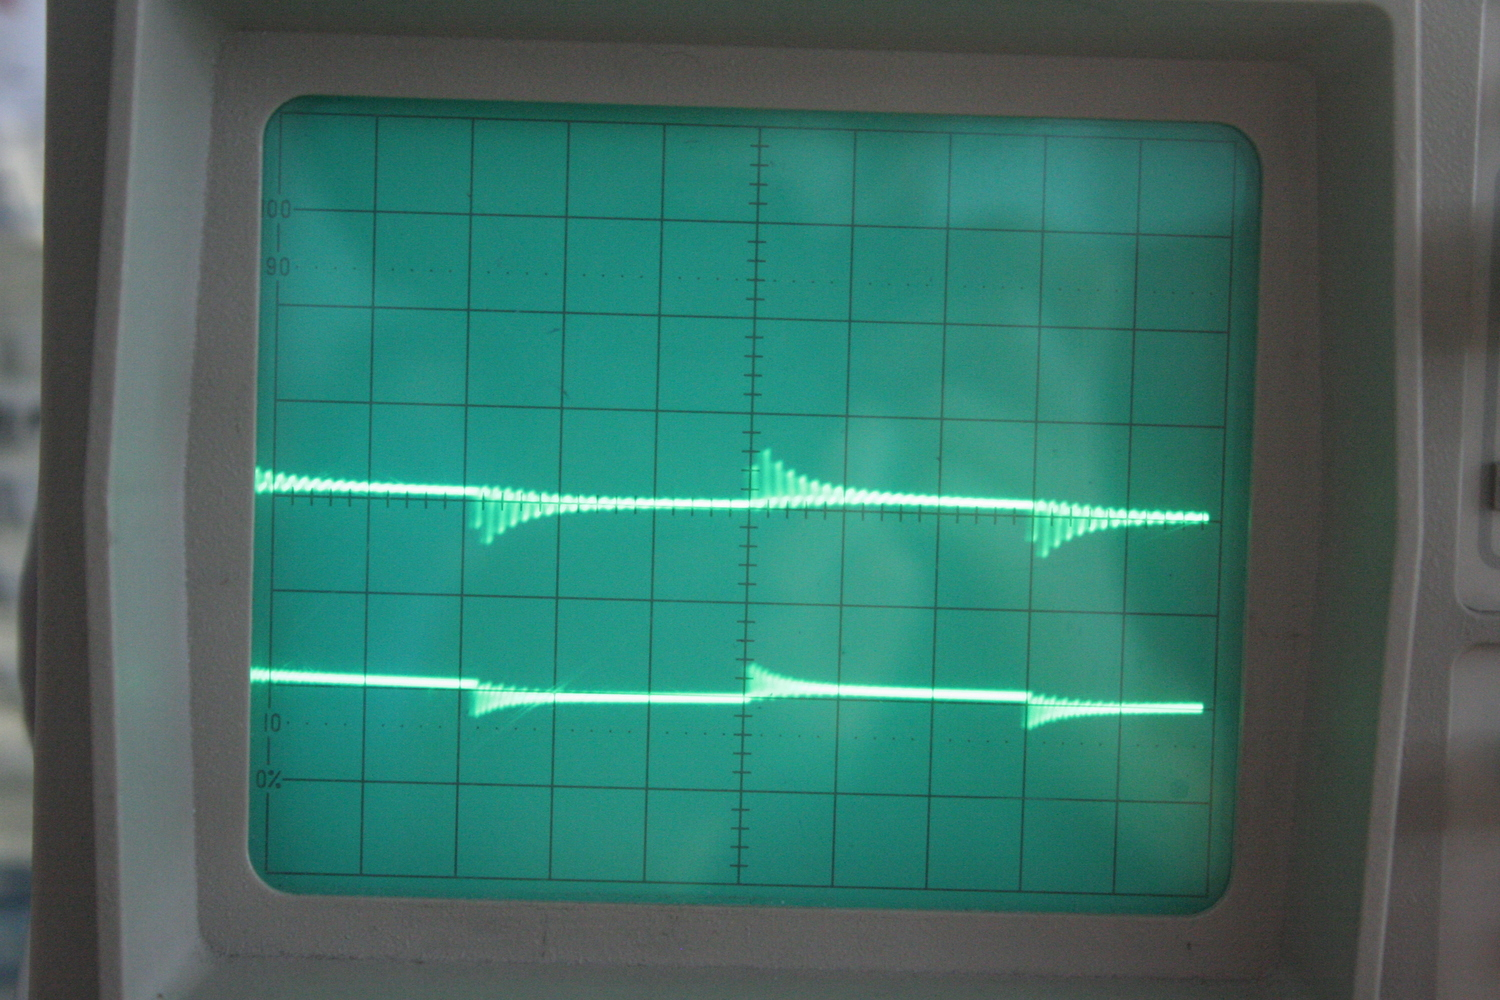
\includegraphics[width=\linewidth]{Fotos/IMG_0756-1500.jpg}
	\end{minipage}
	\caption{%
		Rechteck, Frequenz \SI{200}{\kilo\hertz}, Zeitbasis \SI{1}{\micro\second\per\division}, Verstärkung \SI{5}{\milli\volt\per\division}, externe Triggerung
	}
	\label{fig:0756}
\end{figure}

\begin{figure}
	\centering
	\begin{minipage}{.45\linewidth}
	\end{minipage}
	\hfill
	\begin{minipage}{.45\linewidth}
	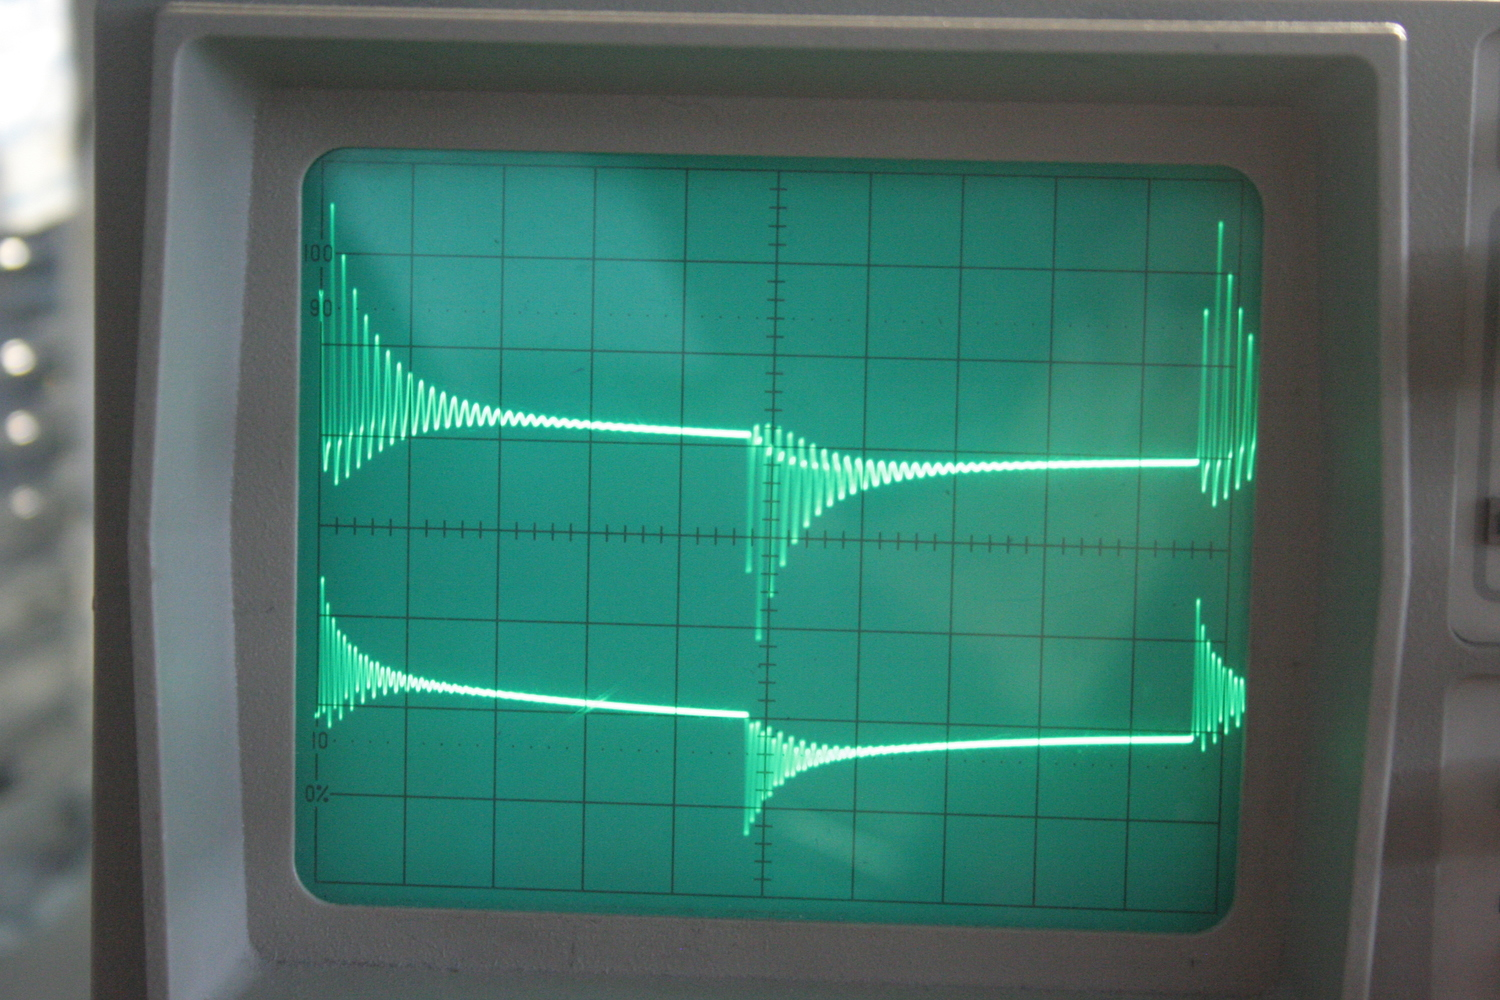
\includegraphics[width=\linewidth]{Fotos/IMG_0757-1500.jpg}
	\end{minipage}
	\caption{%
		Rechteck, Frequenz \SI{1000}{\kilo\hertz}, Zeitbasis \SI{1}{\micro\second\per\division}, Verstärkung \SI{50}{\milli\volt\per\division}, externe Triggerung
	}
	\label{fig:0757}
\end{figure}

Bei näherer Betrachtung (Abbildung \ref{fig:0759}) ist zu erkennen, dass die
obere Linie Zwischenpeaks hat, während die untere dafür richtige Peaks hat. Die
Untere hat kleine und große Peaks. Dips auf Kanal 1 korrespondieren zu großen
Peaks auf Kanal 2.

\begin{figure}
	\centering
	\begin{minipage}{.45\linewidth}
	\end{minipage}
	\hfill
	\begin{minipage}{.45\linewidth}
	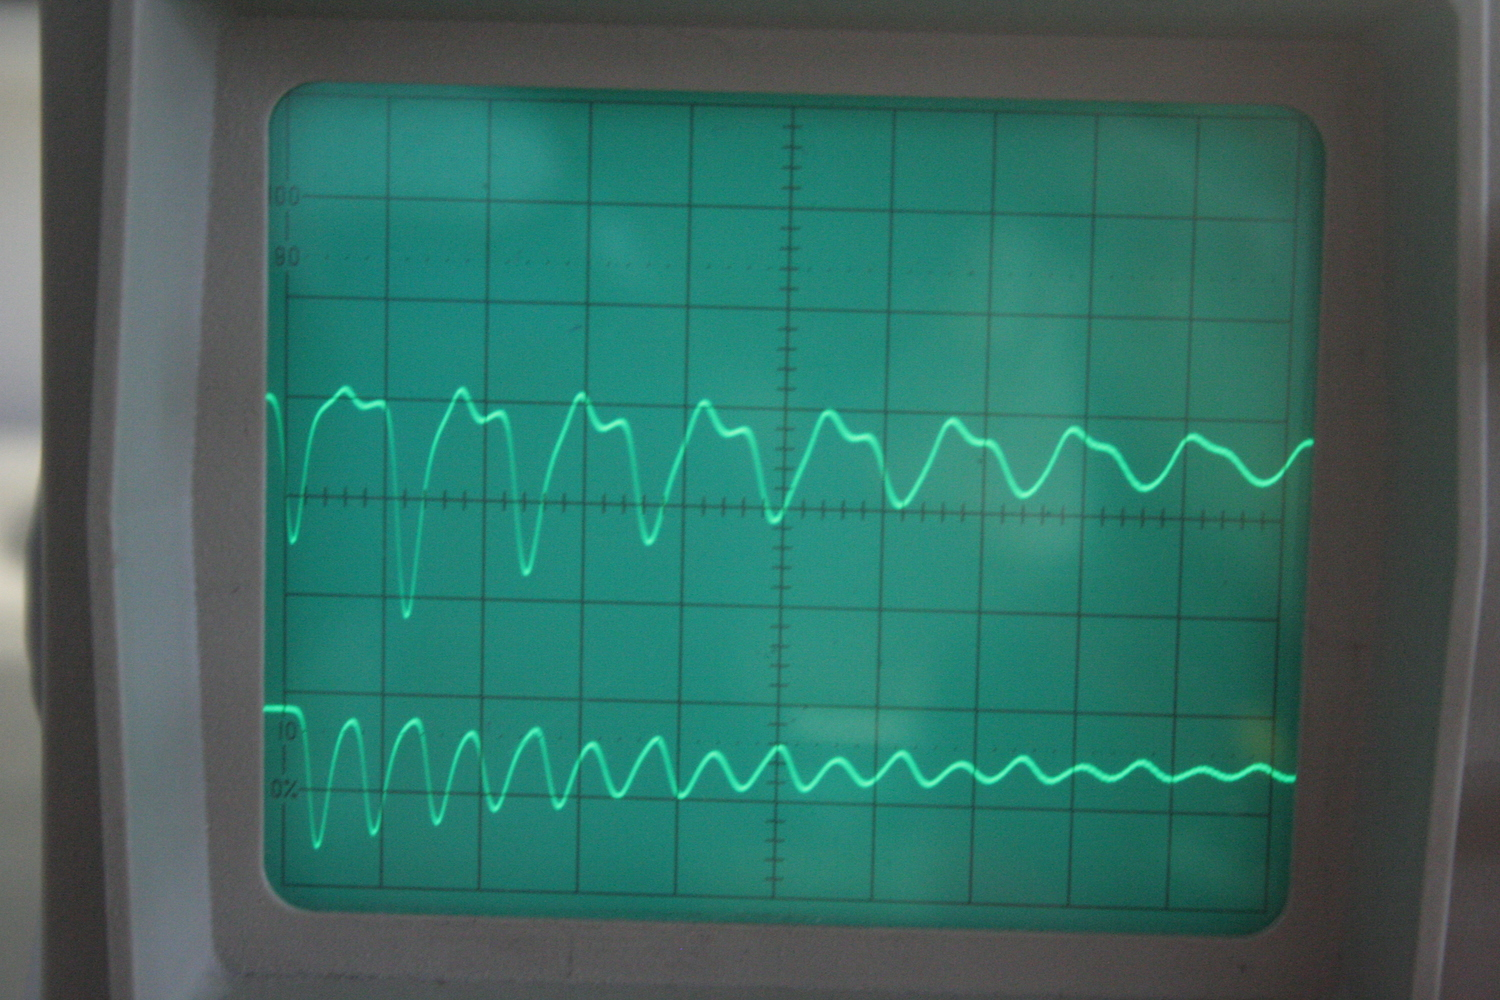
\includegraphics[width=\linewidth]{Fotos/IMG_0759-1500.jpg}
	\end{minipage}
	\caption{%
		Rechteck, Frequenz \SI{1000}{\kilo\hertz},
		Zeitbasis \SI{1}{\micro\second\per\division},
		$\times 10$,
		Verstärkung \SI{50}{\milli\volt\per\division},
		externe Triggerung
	}
	\label{fig:0759}
\end{figure}

\FloatBarrier
\subsection{Versuchsaufgabe 3: Leitungsabschluss, Verzögerungszeit}

Wir schließen das Differenzierglied mit zusätzlichem Widerstand an den
Funktionsgenerator an, den wir auf Rechteck stehen lassen. An das
Differenzierglied kommen:
%
\begin{itemize}
	\item
		Abschlusswiderstand
	\item
		Langes BNC-Kabel (Verzögerungskabel), später mit Anpassungswiderstand
		von $R_\text A = Z$
	\item
		Oszillograph
\end{itemize}

\FloatBarrier
\subsubsection{Teil a}

In Abbildung \ref{fig:0763} und \ref{fig:0765} sind die Oszillogramme ohne und
mit Abschlusswiderstand.

\begin{figure}
	\centering
	\begin{minipage}{.45\linewidth}
	\end{minipage}
	\hfill
	\begin{minipage}{.45\linewidth}
	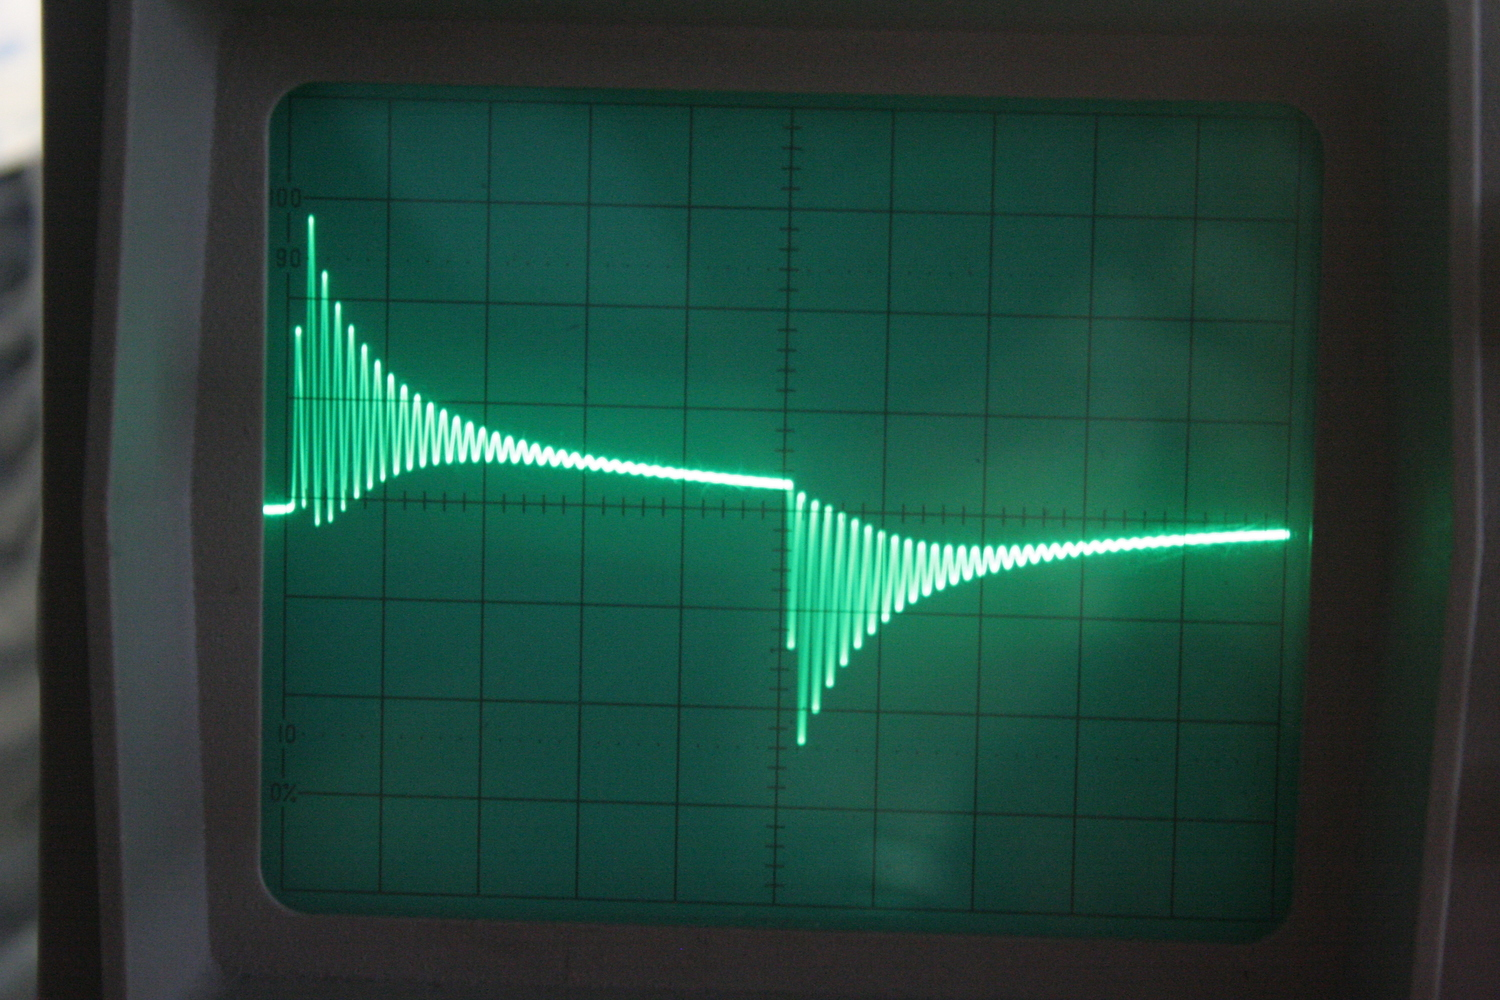
\includegraphics[width=\linewidth]{Fotos/IMG_0763-1500.jpg}
	\end{minipage}
	\caption{%
		Rechteck, Frequenz \SI{200}{\kilo\hertz},
		Zeitbasis \SI{.05}{\micro\second\per\division},
		Verstärkung \SI{50}{\milli\volt\per\division},
		externe Triggerung
	}
	\label{fig:0763}
\end{figure}

\begin{figure}
	\centering
	\begin{minipage}{.45\linewidth}
	\end{minipage}
	\hfill
	\begin{minipage}{.45\linewidth}
	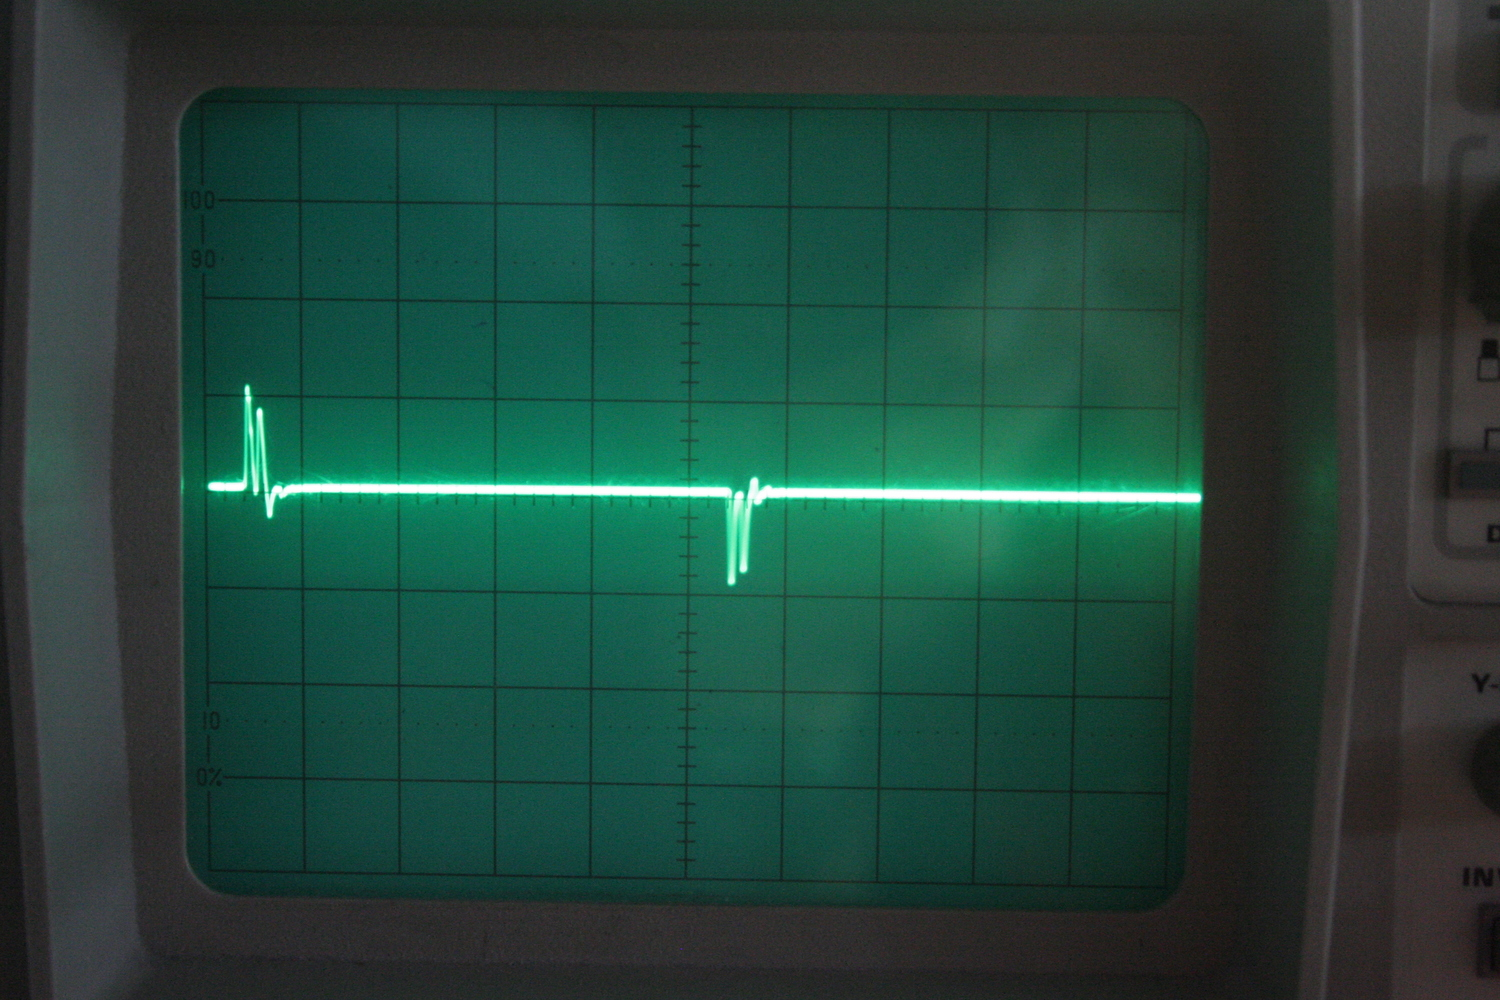
\includegraphics[width=\linewidth]{Fotos/IMG_0765-1500.jpg}
	\end{minipage}
	\caption{%
		Rechteck, Frequenz \SI{200}{\kilo\hertz},
		Zeitbasis \SI{.5}{\micro\second\per\division},
		Verstärkung \SI{50}{\milli\volt\per\division},
		externe Triggerung
	}
	\label{fig:0765}
\end{figure}

\FloatBarrier
\subsubsection{Teil b}

In Abbildung \ref{fig:0764} und \ref{fig:0766} sind die Oszillogramme ohne und
mit Abschlusswiderstand, mit zehnfacher Vergrößerung.

\begin{figure}
	\centering
	\begin{minipage}{.45\linewidth}
	\end{minipage}
	\hfill
	\begin{minipage}{.45\linewidth}
	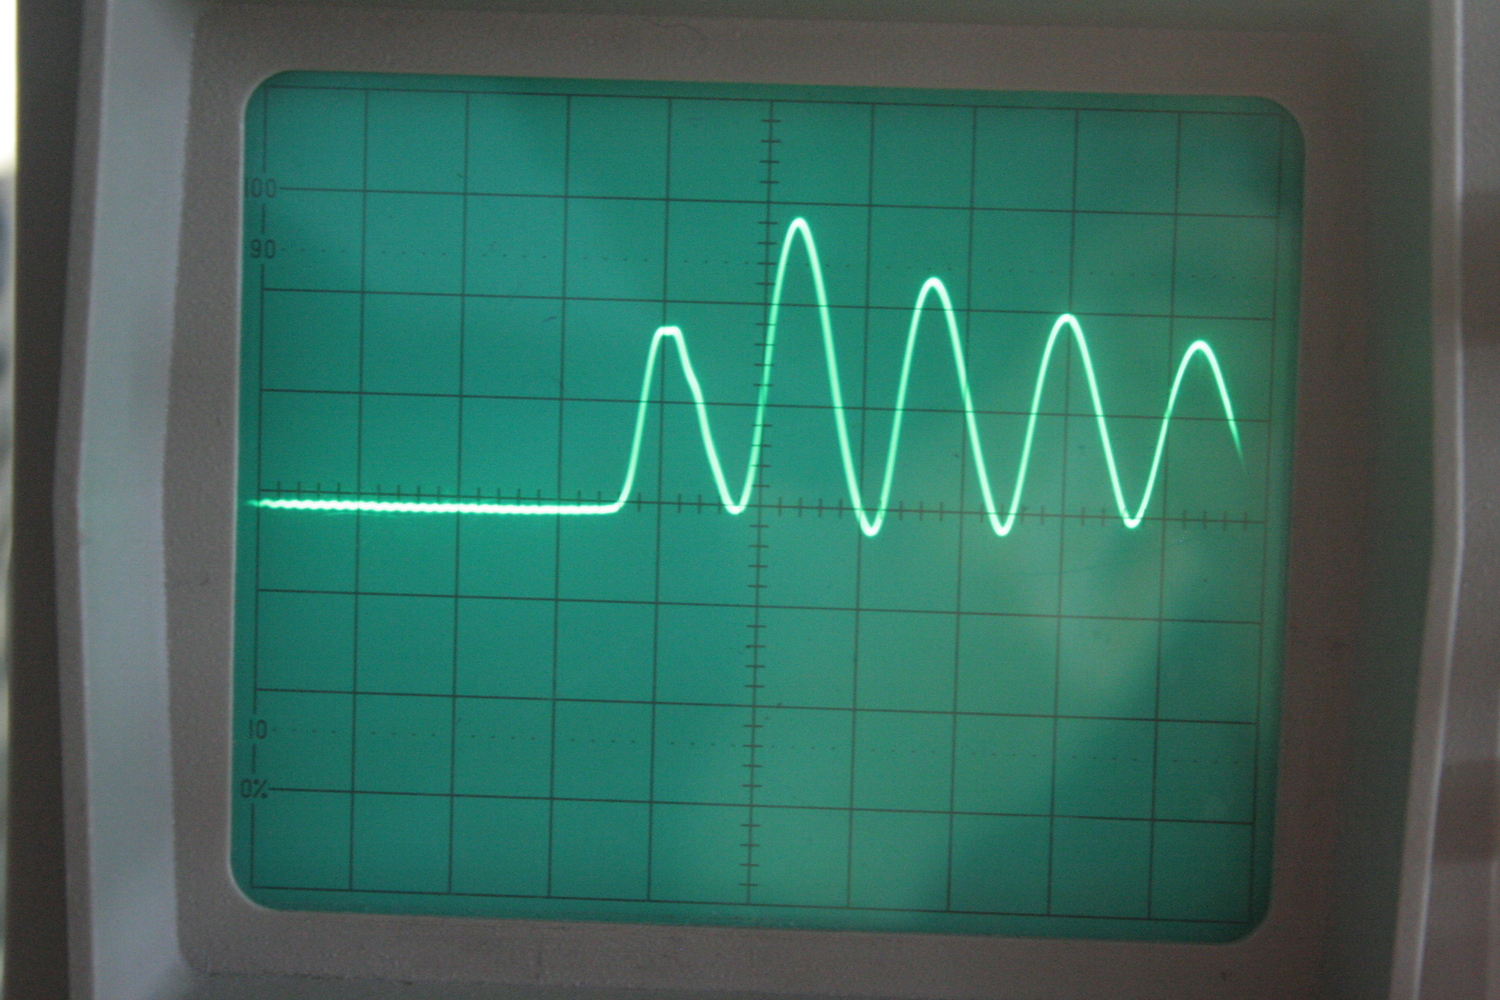
\includegraphics[width=\linewidth]{Fotos/IMG_0764-1500.jpg}
	\end{minipage}
	\caption{%
		Rechteck, Frequenz \SI{200}{\kilo\hertz},
		Zeitbasis \SI{.05}{\micro\second\per\division},
		Verstärkung \SI{50}{\milli\volt\per\division},
		externe Triggerung
	}
	\label{fig:0764}
\end{figure}

\begin{figure}
	\centering
	\begin{minipage}{.45\linewidth}
	\end{minipage}
	\hfill
	\begin{minipage}{.45\linewidth}
	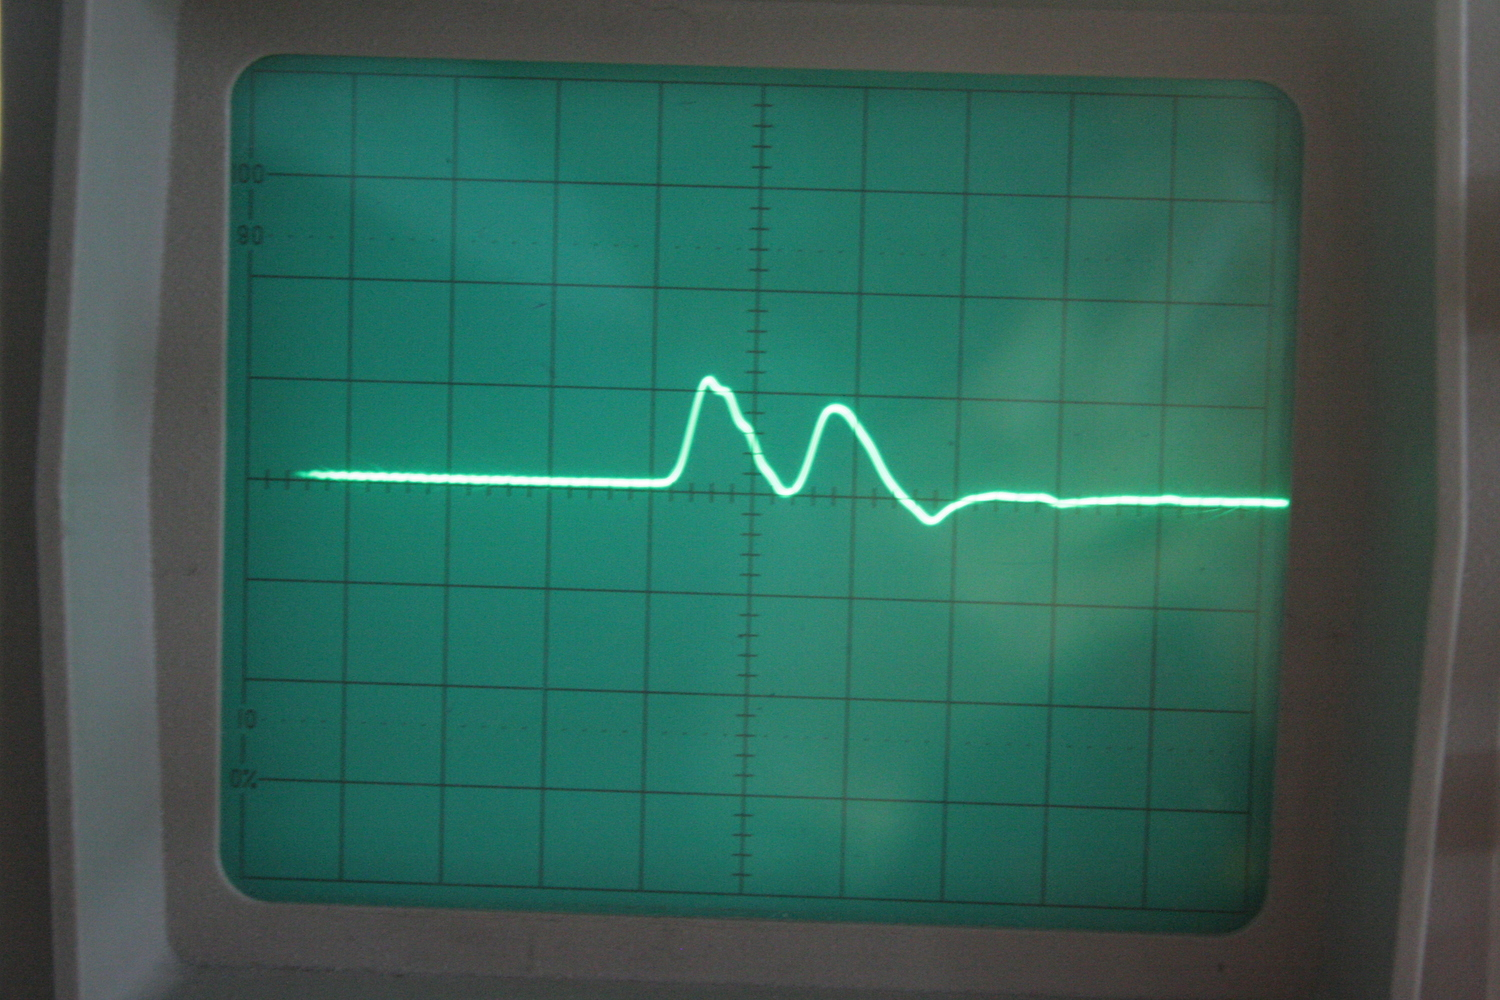
\includegraphics[width=\linewidth]{Fotos/IMG_0766-1500.jpg}
	\end{minipage}
	\caption{%
		Rechteck, Frequenz \SI{200}{\kilo\hertz},
		Zeitbasis \SI{.05}{\micro\second\per\division},
		Verstärkung \SI{50}{\milli\volt\per\division},
		externe Triggerung
	}
	\label{fig:0766}
\end{figure}

\FloatBarrier
\subsubsection{Teil c}

In Abbildung \ref{fig:0767} ist das Oszillogramm ohne Anpassung, in Abbildung
\ref{fig:0786} mit Anpassung gezeigt.

\begin{figure}
	\centering
	\begin{minipage}{.45\linewidth}
	\end{minipage}
	\hfill
	\begin{minipage}{.45\linewidth}
	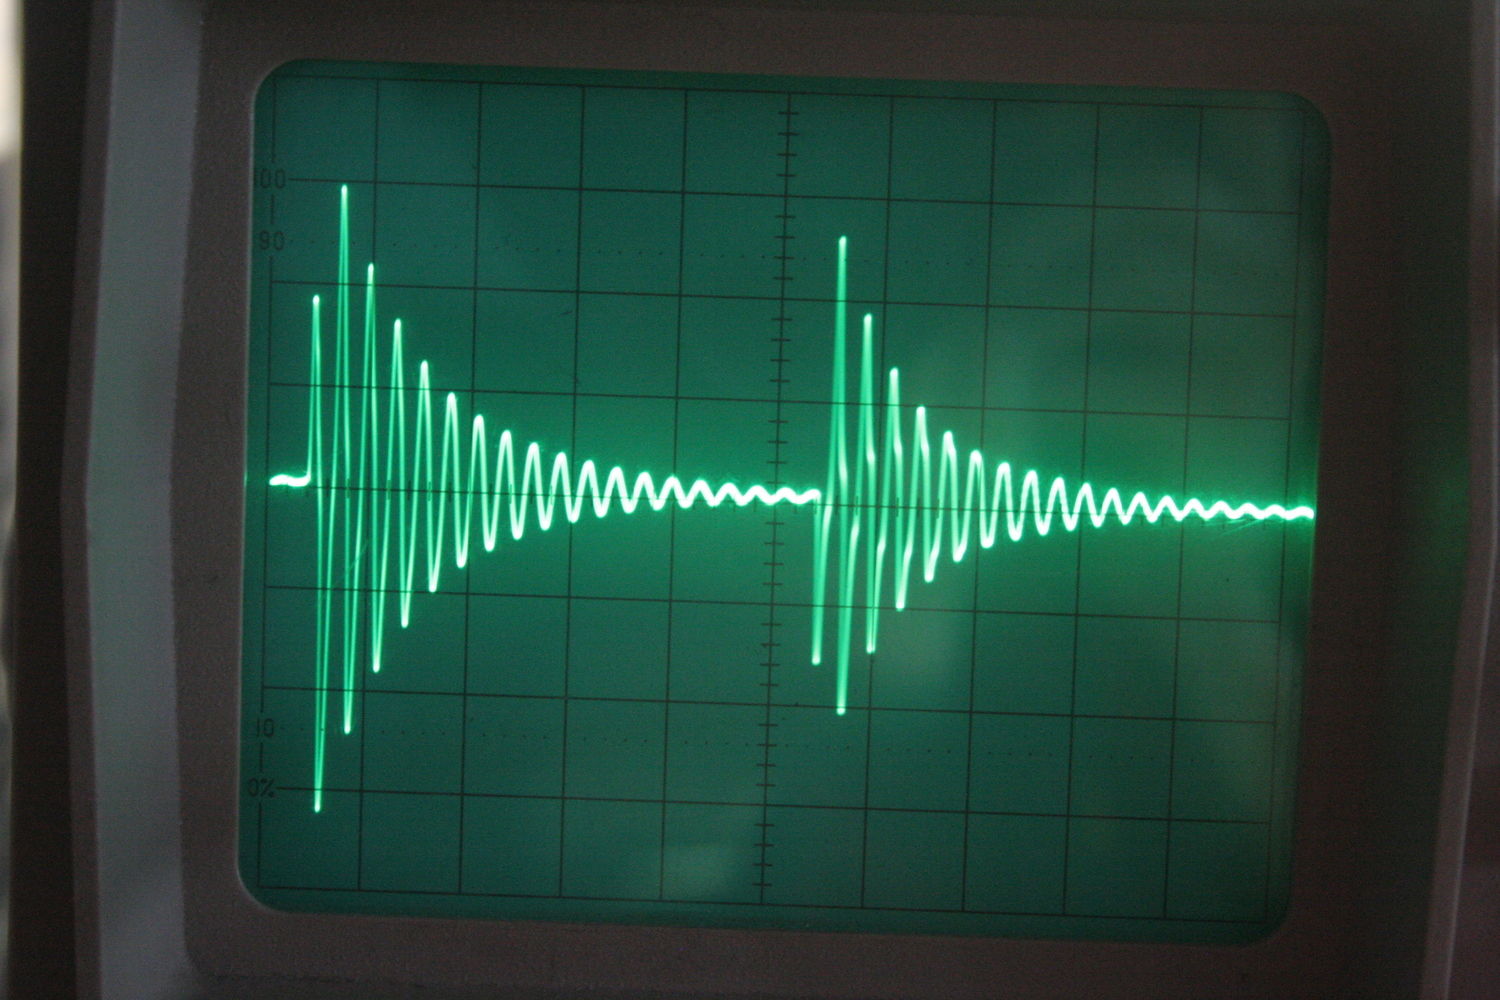
\includegraphics[width=\linewidth]{Fotos/IMG_0767-1500.jpg}
	\end{minipage}
	\caption{%
		Rechteck, Frequenz \SI{200}{\kilo\hertz},
		Zeitbasis \SI{.5}{\micro\second\per\division},
		Verstärkung \SI{50}{\milli\volt\per\division},
		externe Triggerung
	}
	\label{fig:0767}
\end{figure}

\begin{figure}
	\centering
	\begin{minipage}{.45\linewidth}
	\end{minipage}
	\hfill
	\begin{minipage}{.45\linewidth}
	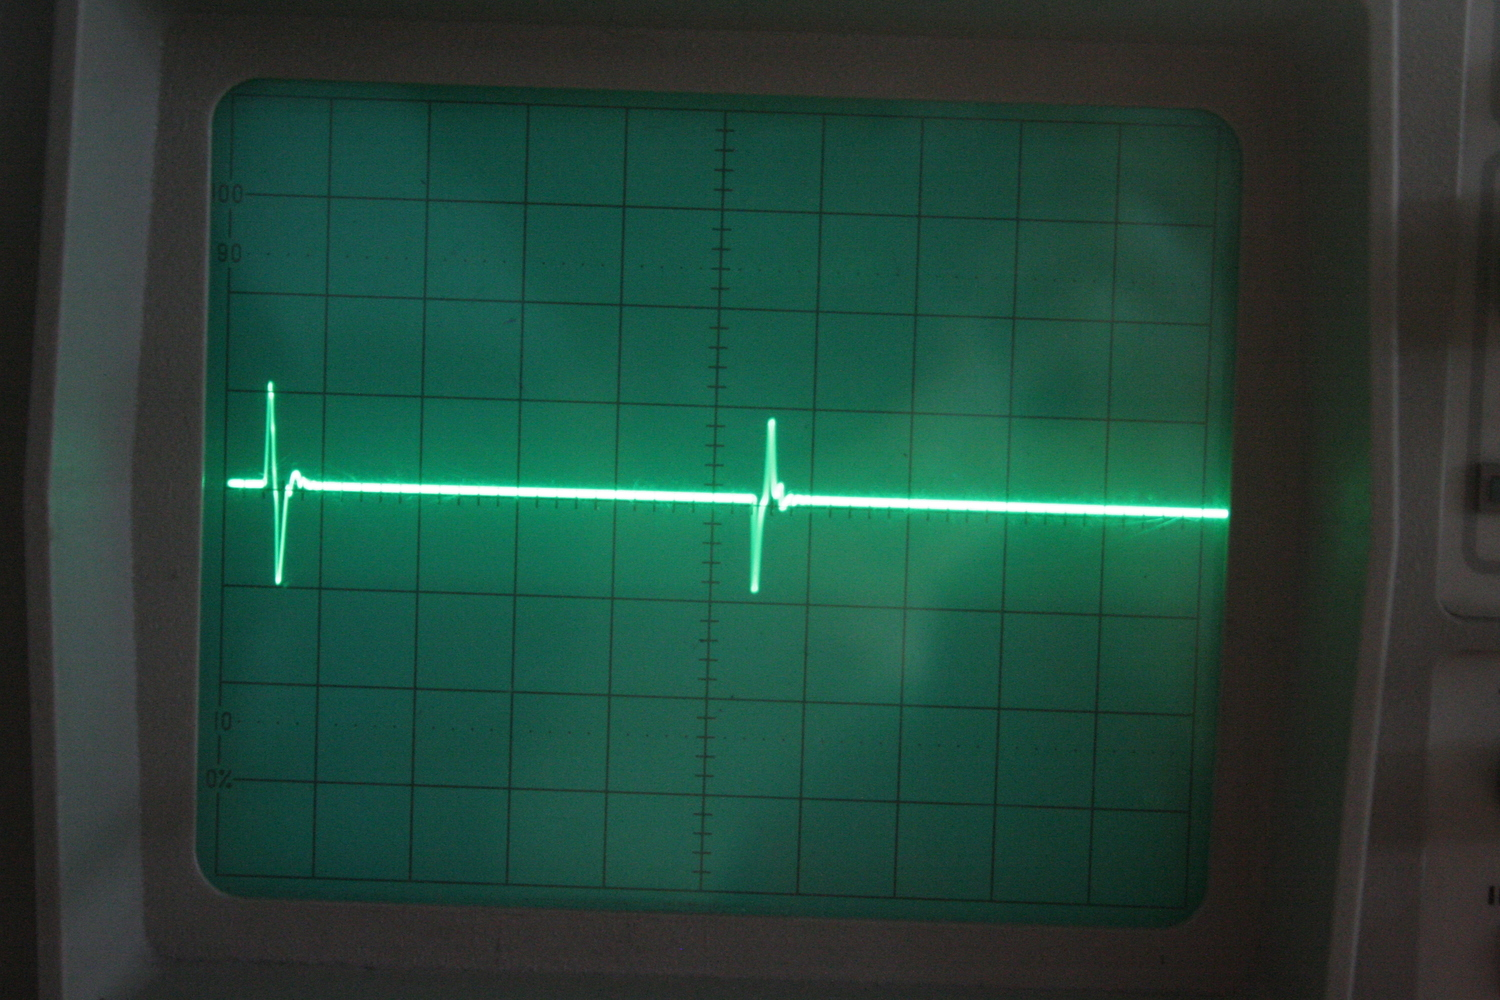
\includegraphics[width=\linewidth]{Fotos/IMG_0768-1500.jpg}
	\end{minipage}
	\caption{%
		Rechteck, Frequenz \SI{200}{\kilo\hertz},
		Zeitbasis \SI{.5}{\micro\second\per\division},
		Verstärkung \SI{50}{\milli\volt\per\division},
		externe Triggerung
	}
	\label{fig:0768}
\end{figure}

\FloatBarrier
\subsubsection{Teil d}

Ohne Anpassungswiderstand in Abbildung \ref{fig:0769}. Zur Illustration sind
noch höhere Frequenzen in den Abbildungen \ref{fig:0770} und \ref{fig:0771}
gezeigt.

\begin{figure}
	\centering
	\begin{minipage}{.45\linewidth}
	\end{minipage}
	\hfill
	\begin{minipage}{.45\linewidth}
	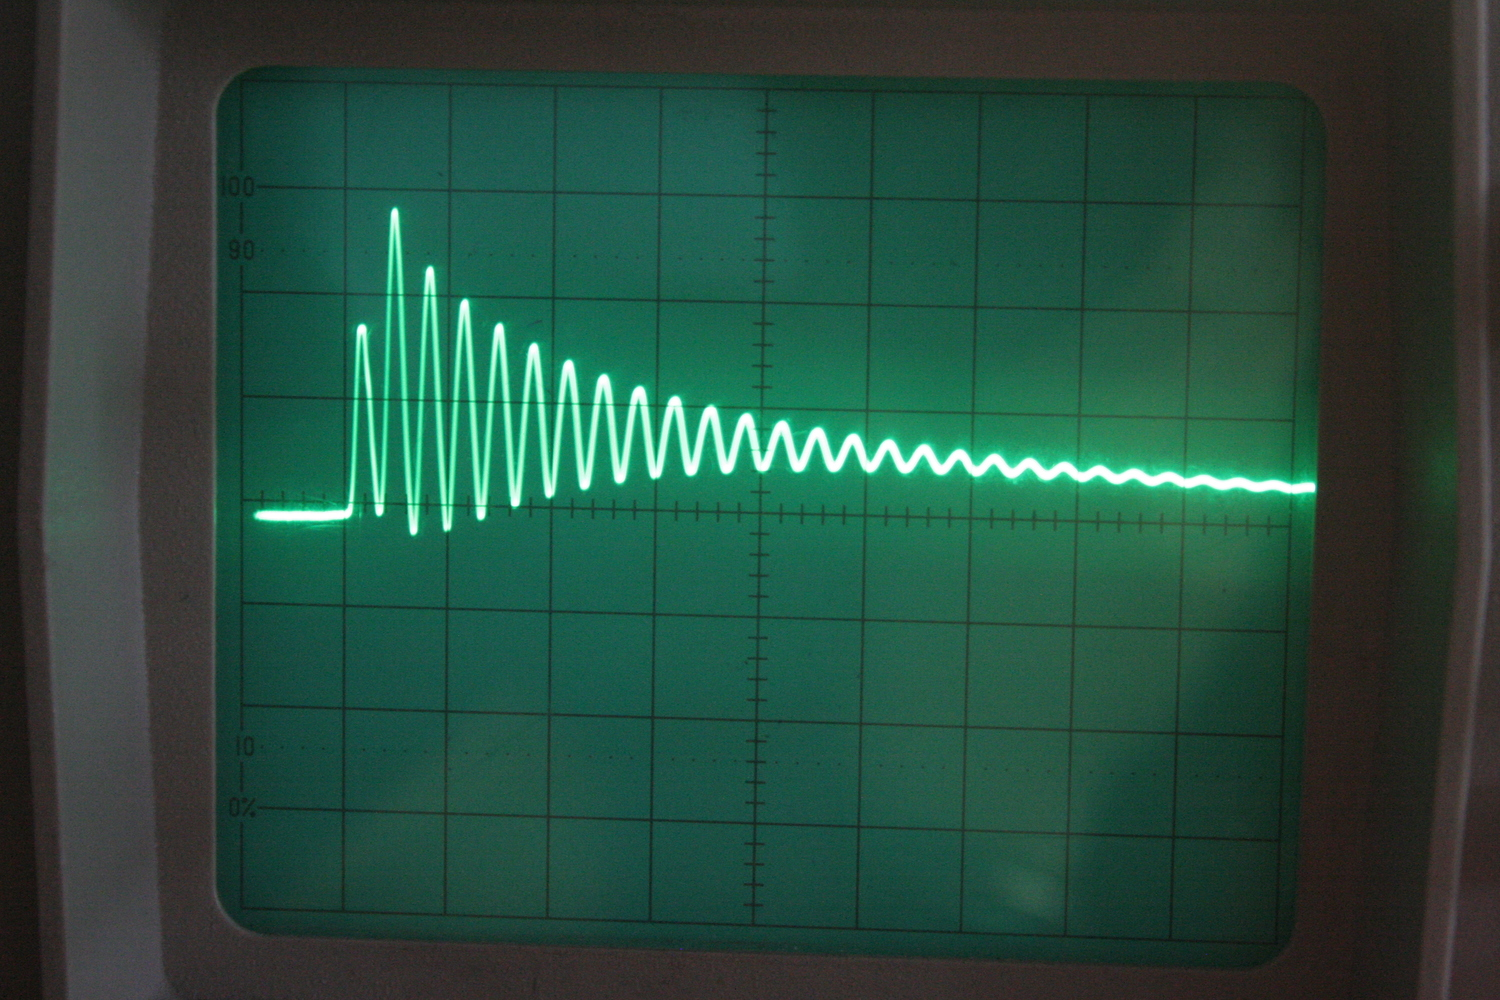
\includegraphics[width=\linewidth]{Fotos/IMG_0769-1500.jpg}
	\end{minipage}
	\caption{%
		Rechteck, Frequenz \SI{200}{\kilo\hertz},
		Zeitbasis \SI{.2}{\micro\second\per\division},
		Verstärkung \SI{50}{\milli\volt\per\division},
		externe Triggerung
	}
	\label{fig:0769}
\end{figure}

\begin{figure}
	\centering
	\begin{minipage}{.45\linewidth}
	\end{minipage}
	\hfill
	\begin{minipage}{.45\linewidth}
	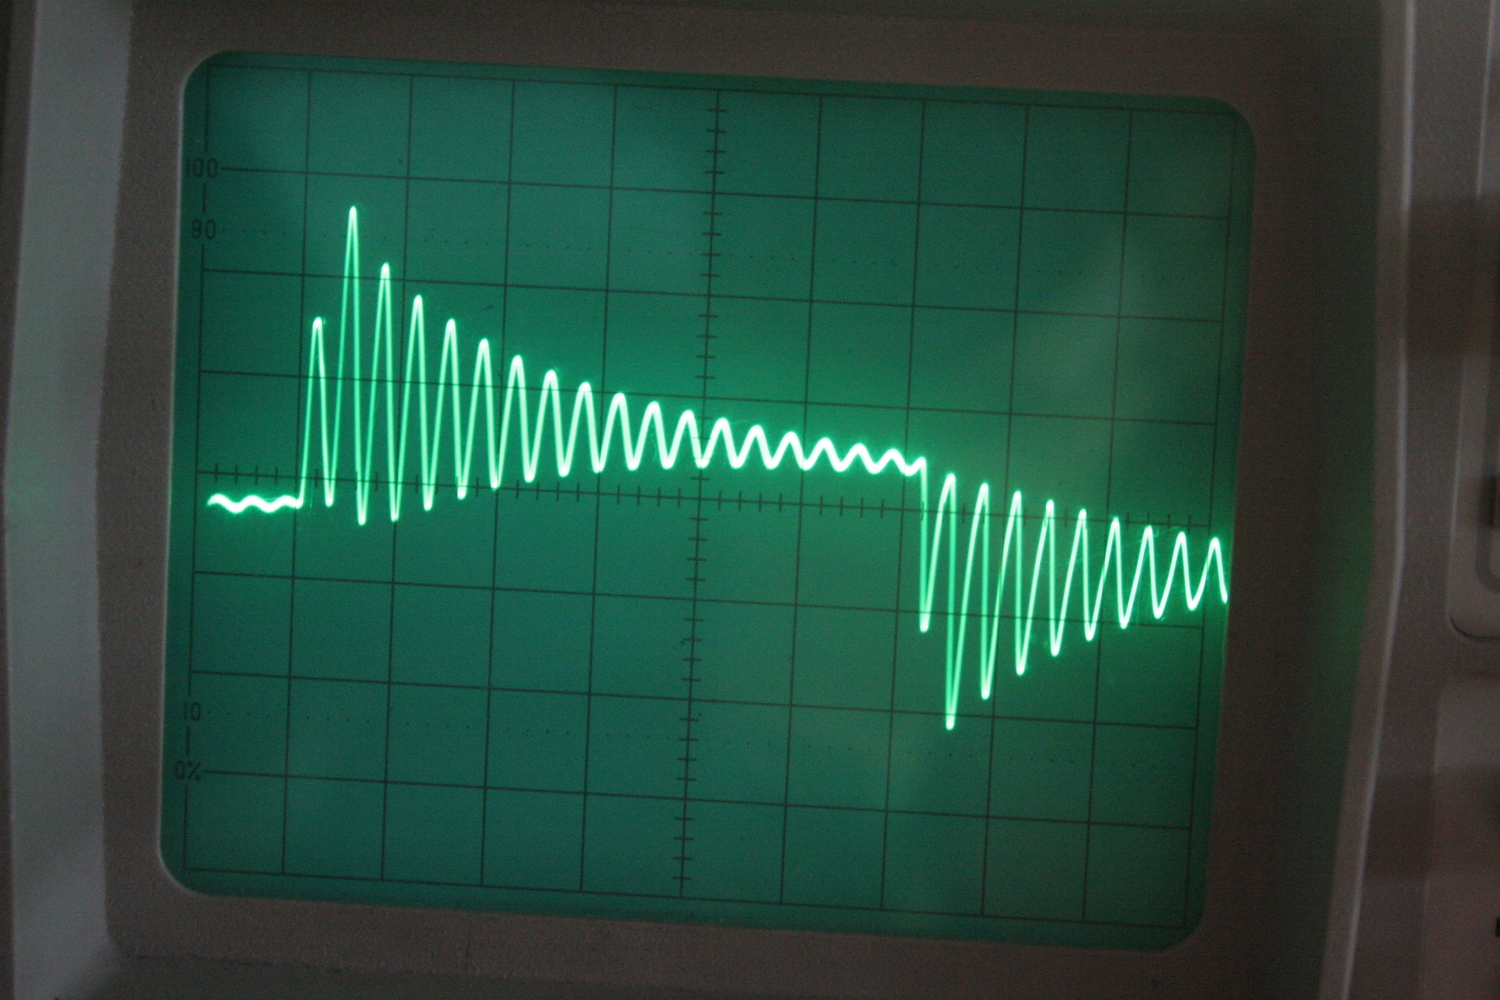
\includegraphics[width=\linewidth]{Fotos/IMG_0770-1500.jpg}
	\end{minipage}
	\caption{%
		Rechteck, Frequenz \SI{400}{\kilo\hertz},
		Zeitbasis \SI{.2}{\micro\second\per\division},
		Verstärkung \SI{50}{\milli\volt\per\division},
		externe Triggerung
	}
	\label{fig:0770}
\end{figure}

\begin{figure}
	\centering
	\begin{minipage}{.45\linewidth}
	\end{minipage}
	\hfill
	\begin{minipage}{.45\linewidth}
	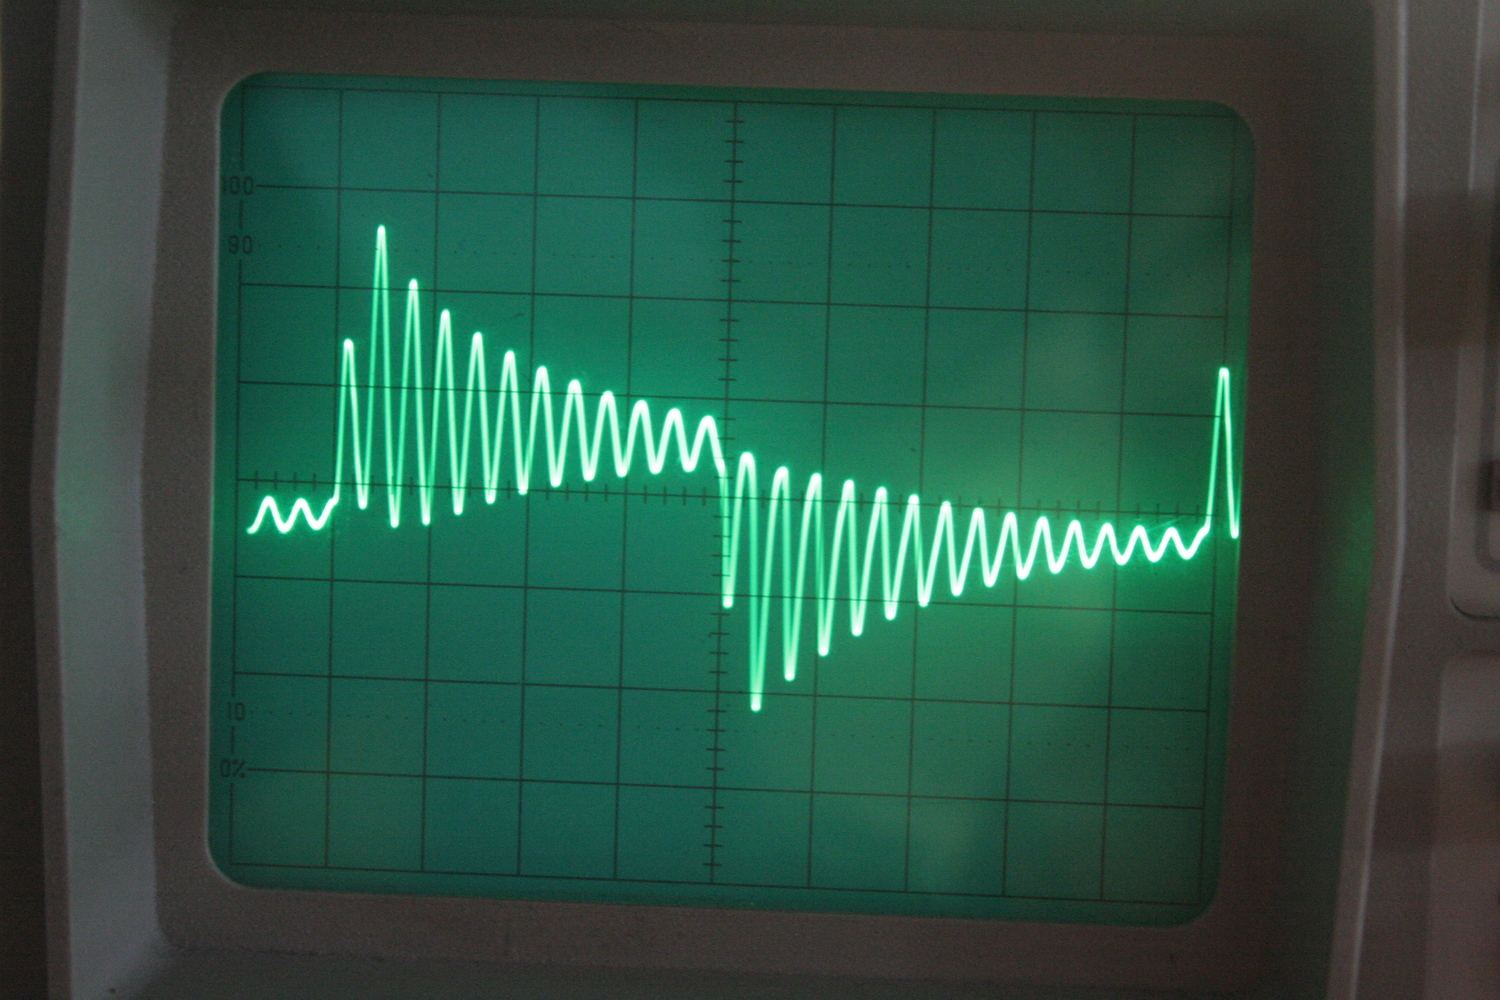
\includegraphics[width=\linewidth]{Fotos/IMG_0771-1500.jpg}
	\end{minipage}
	\caption{%
		Rechteck, Frequenz \SI{600}{\kilo\hertz},
		Zeitbasis \SI{.2}{\micro\second\per\division},
		Verstärkung \SI{50}{\milli\volt\per\division},
		externe Triggerung
	}
	\label{fig:0771}
\end{figure}

Wir lesen aus dem Oszillogramm ab 12 Peaks auf 4 Kästchen ab. Die
Zeitauflösung ist auf \SI{.2}{\micro\second\per\division}, eingestellt. Somit
ergibt sich eine Frequenz von $\nu = \SI{<< nu >>}{\hertz}$ und eine Periode
von $T = \SI{<< T >>}\second$. Dies ist die Zeit, die das Signal braucht, um
die \SI{<< kabel_length >>}{\meter} \emph{zweimal} zurückzulegen. Daraus folgt
eine spezifische Verzögerungszeit von \SI{<< spez_verz >>}{\second\per\meter}.
Der Literaturwert für RG-58C/U Kabel ist \SI{5}{\nano\second\per\meter}, dies
passt also gut.

Bei Kurzschluss des Verzögerungskabels halbiert sich die Anzahl der Peaks, jedoch wird das Signal jetzt symmetrisch. Dies kommt daher, dass die Reflexion jetzt am festen Ende ist, so dass die Amplitude negiert wird. Daher ist jetzt nicht mehr Peak, Null, Peak, sondern Plus, Minus, Plus abzulesen. Siehe Abbildung \ref{fig:0772}.

\begin{figure}
	\centering
	\begin{minipage}{.45\linewidth}
	\end{minipage}
	\hfill
	\begin{minipage}{.45\linewidth}
	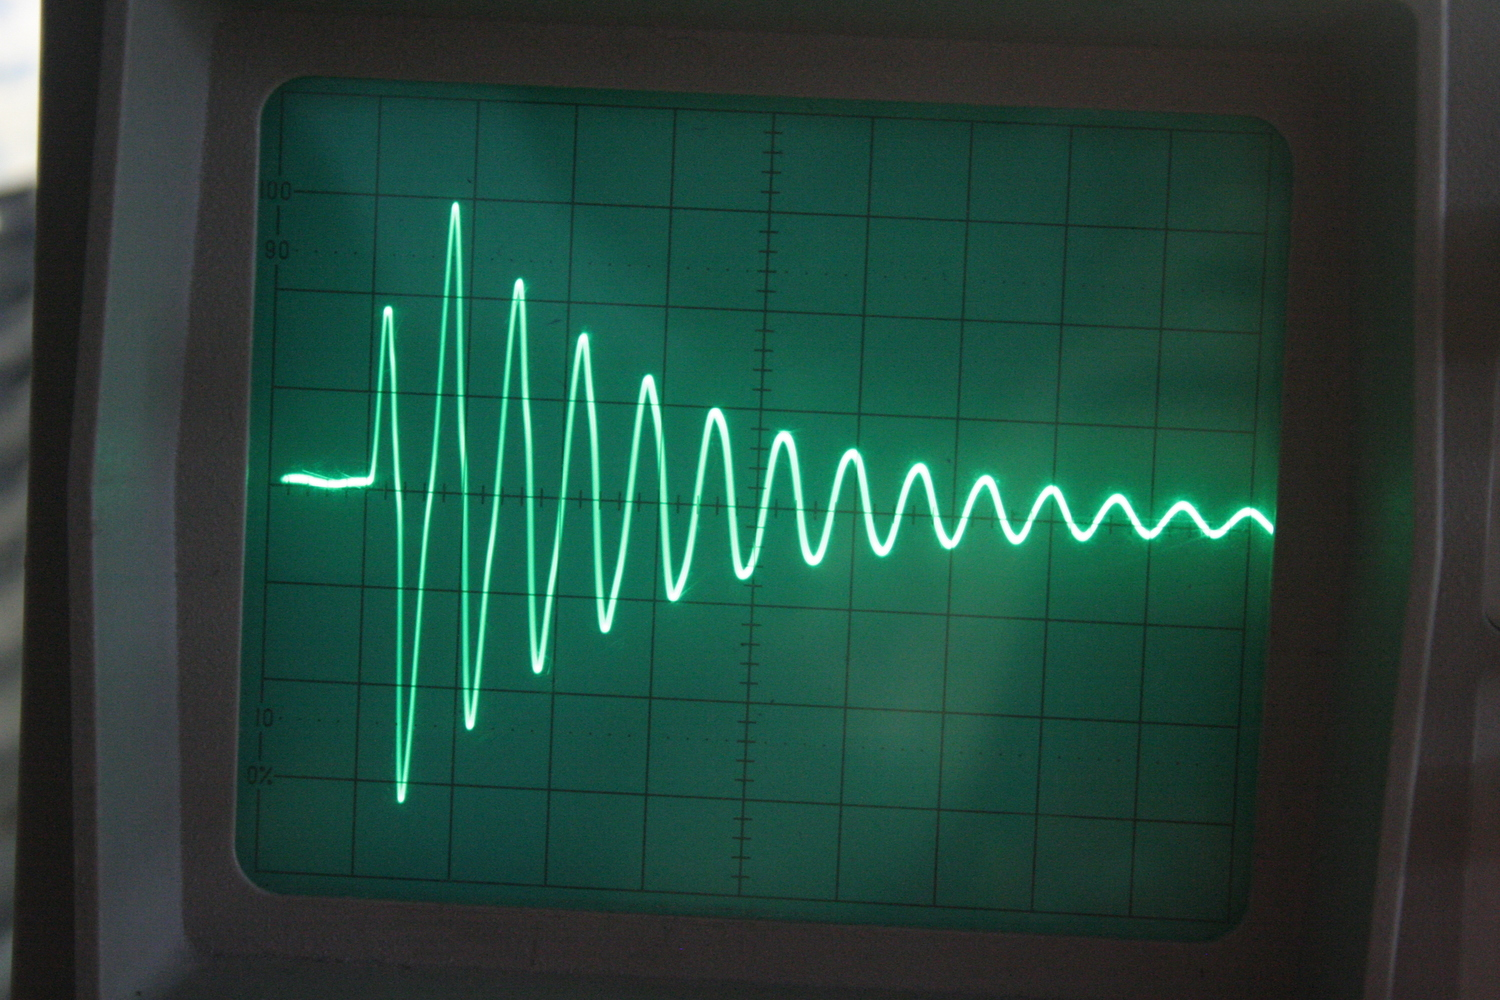
\includegraphics[width=\linewidth]{Fotos/IMG_0772-1500.jpg}
	\end{minipage}
	\caption{%
		Rechteck, Frequenz \SI{200}{\kilo\hertz},
		Zeitbasis \SI{.2}{\micro\second\per\division},
		Verstärkung \SI{50}{\milli\volt\per\division},
		externe Triggerung
	}
	\label{fig:0772}
\end{figure}

Bei Abschluss erwarten wir, dass die Reflexionen verschwinden und nur noch der
eine Peak vom Differenzierer zu sehen ist. So ist es auch.

\FloatBarrier
\subsection{Versuchsaufgabe 4: Klippkabel, Dämpfung}

\FloatBarrier
\subsubsection{Teil a}

Wir lassen das Verzögerungskabel zunächst offen. Dadurch werden die Wellen
offen reflektiert, also mit gleich bleibender Amplitude. Die reflektierte
Teilwelle verbindet sich einfach additiv mit der normalen Welle, die gerade im
Funktionsgenerator generiert wird. Der Effekt ist, dass am Anfang und am Ende
die Amplitude des Signals etwas halb so groß ist. Das passende Oszillogramm ist
in Abbildung \ref{fig:0773} gezeigt. Wenn man genau hinschaut, ist auch zu
sehen, dass die Stufe bei vor der positiven Halbwelle etwas höher ist, als vor
der negativen Halbwelle. Dies liegt daran, dass das Verzögerungskabel eine
Dämpfung hat und somit die zweite Hälfte des Signals weniger als die halbe
Amplitude hat.

\begin{figure}
	\centering
	\begin{minipage}{.45\linewidth}
	\end{minipage}
	\hfill
	\begin{minipage}{.45\linewidth}
	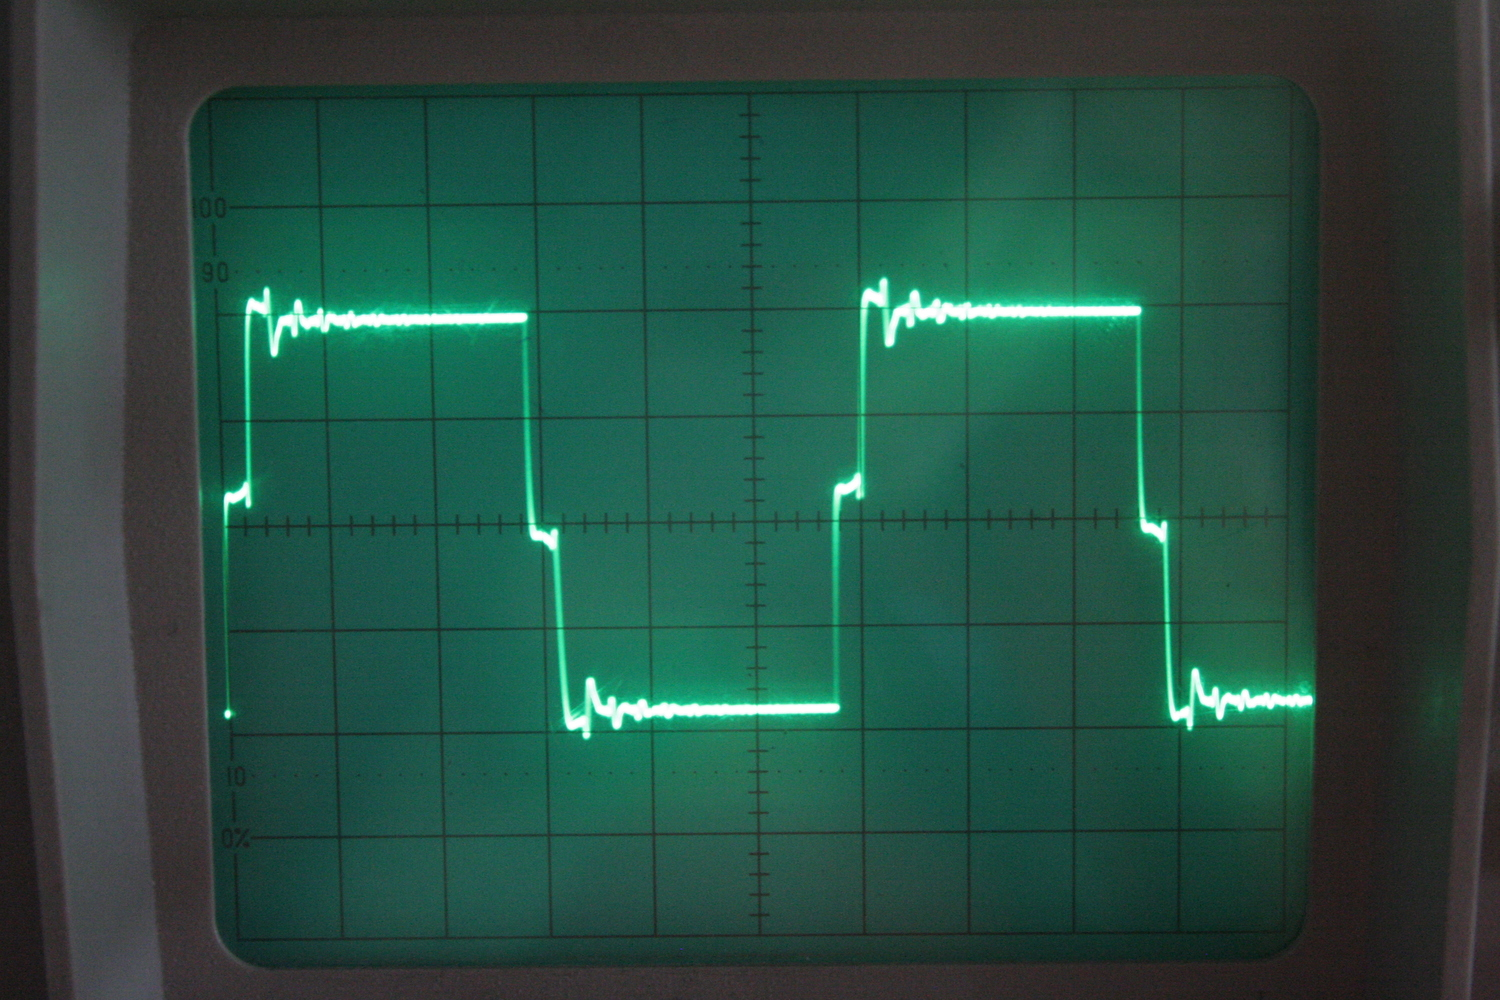
\includegraphics[width=\linewidth]{Fotos/IMG_0773-1500.jpg}
	\end{minipage}
	\caption{%
		Rechteck, Frequenz \SI{200}{\kilo\hertz},
		Zeitbasis \SI{10}{\micro\second\per\division},
		Verstärkung \SI{5}{\volt\per\division},
		externe Triggerung
	}
	\label{fig:0773}
\end{figure}

\FloatBarrier
\subsubsection{Teil b}

Wir schließen das Klippkabel nun kurz. Das Oszillogramm ist in Abbildung
\ref{fig:0774}. Ähnlich wie vorher wird die Welle im Verzögerungskabel
reflektiert, jedoch am festen Ende mit Negierung der Amplitude. Die zweite
Hälfte wird also nun nach der Verzögerungszeit von der ersten Hälfte
\emph{subtrahiert}. Dadurch wird der Impuls geklippt.

\begin{figure}
	\centering
	\begin{minipage}{.45\linewidth}
	\end{minipage}
	\hfill
	\begin{minipage}{.45\linewidth}
	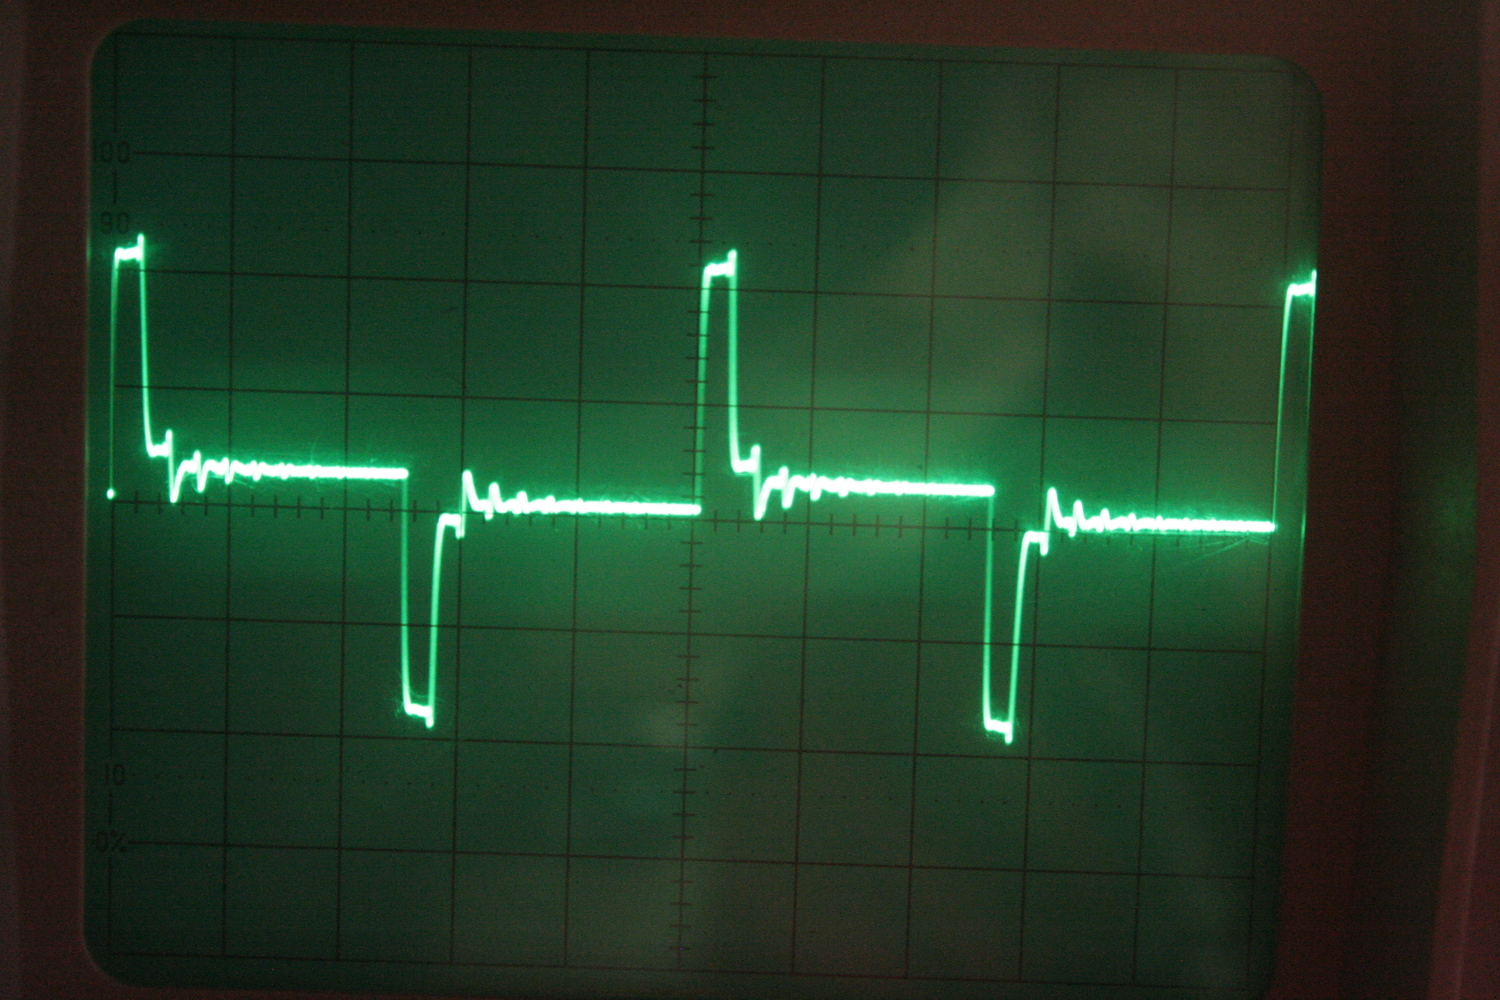
\includegraphics[width=\linewidth]{Fotos/IMG_0774-1500.jpg}
	\end{minipage}
	\caption{%
		Rechteck, Frequenz \SI{200}{\kilo\hertz},
		Zeitbasis \SI{10}{\micro\second\per\division},
		Verstärkung \SI{5}{\volt\per\division},
		externe Triggerung
	}
	\label{fig:0774}
\end{figure}

\FloatBarrier
\subsubsection{Teil c}

Wir verändern nun die Frequenz. Die Abstände der einzelnen Pulse verändern
sich. Die Länge des beschnittenen Pulses bleibt jedoch gleich, da diese Länge
nur von der Verzögerungszeit des Klippkabels abhängt.

\FloatBarrier
\subsubsection{Teil d}

Nun verlängern wir das Klippkabel auf \SI{2.1}{\meter}, in dem wir drei der
vorhandenen zusammenhängen. Das Oszillogramm ist in Abbildung \ref{fig:0775}
gezeigt. Die Länge der geklippten Impulse wird durch die Verzögerungszeit des
kominierten Kabels bestimmt. Der Mechanismus ist der im vorigen Aufgabenteil
beschriebene.

\begin{figure}
	\centering
	\begin{minipage}{.45\linewidth}
	\end{minipage}
	\hfill
	\begin{minipage}{.45\linewidth}
	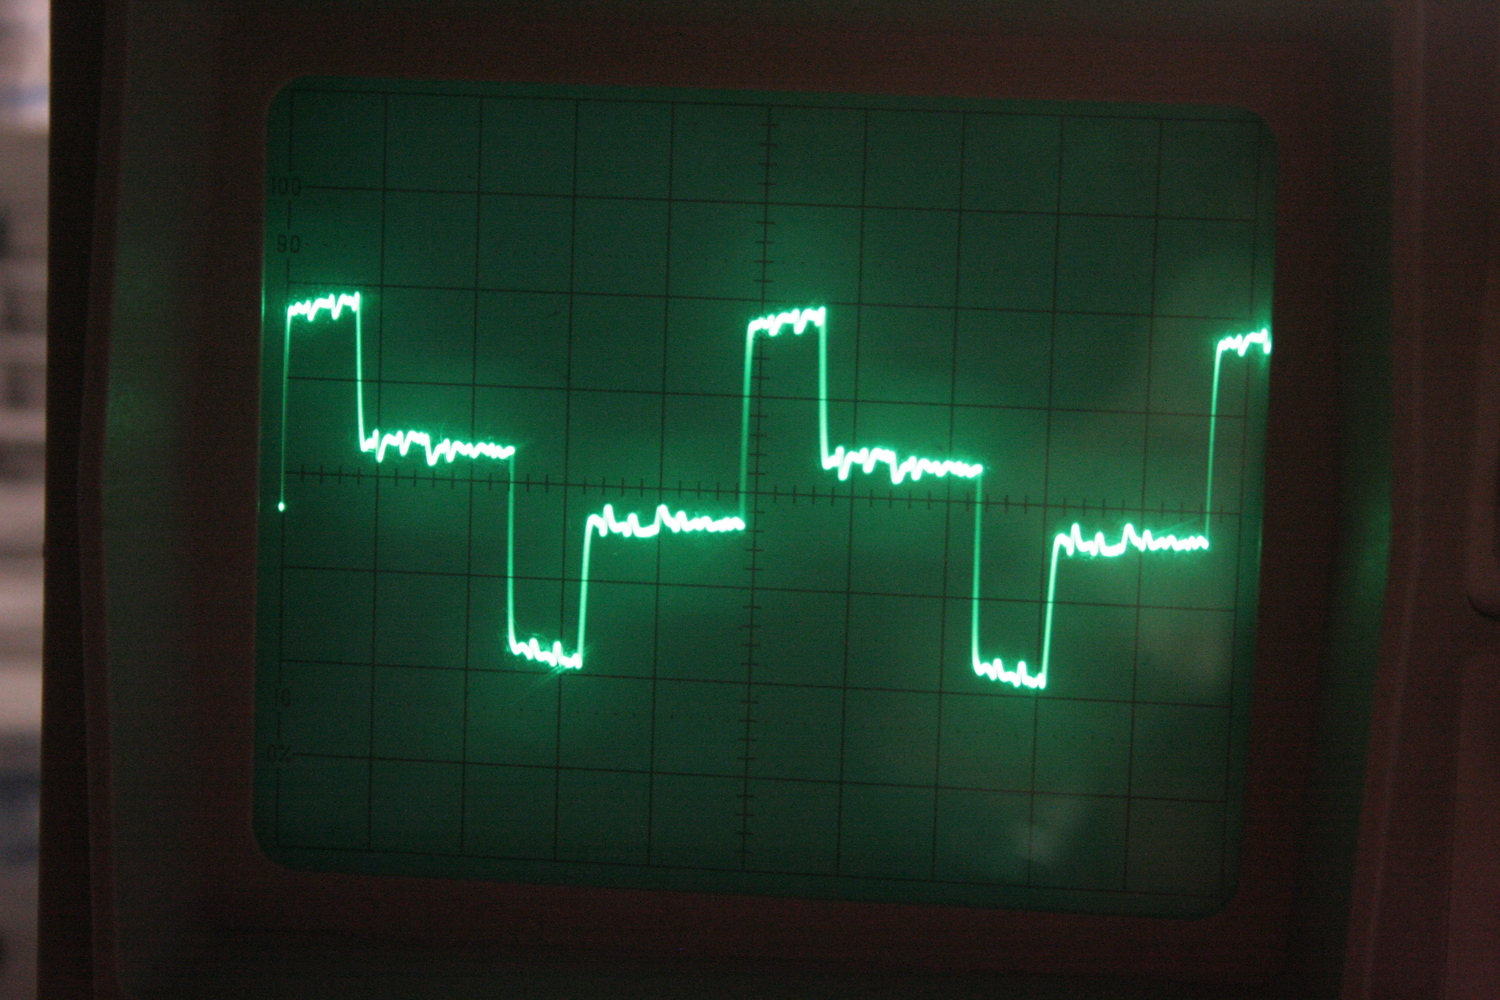
\includegraphics[width=\linewidth]{Fotos/IMG_0775-1500.jpg}
	\end{minipage}
	\caption{%
		Rechteck, Frequenz \SI{200}{\kilo\hertz},
		Zeitbasis \SI{10}{\micro\second\per\division},
		Verstärkung \SI{5}{\volt\per\division},
		externe Triggerung
	}
	\label{fig:0775}
\end{figure}

Wir lesen ein Verhältnis von $9 : 2$ ab.

\FloatBarrier
\subsection{Versuchsaufgabe 5: \SI{50}{\ohm} Kabel RG-58 C/U}

\subsubsection{Teil a}

\begin{problem}
	Warum macht sich eine kleine Bandbreite besonders bei der Übertragung von
	Rechtecksignalen bemerkbar?
\end{problem}

Entwickelt man ein Rechtecksignal in eine Fourierreihe, so fallen die
Amplituden der hohen Frequenzen nur langsam ab, weil die Funktion nicht
besonders glatt ist. Dies bedeutet, dass sehr viele hohe Frequenzen mit
einbezogen werden müssen, damit die Summe wie ein Rechteck aussieht. Bei einer
kleinen Bandbreite ist allerdings genau dies das Problem: Hohe Frequenzen
werden abgeschnitten, da sie besonders gedämpft werden. So wird das Rechteck an
den Ecken etwas abgerundet.

\begin{figure}
	\centering
	\begin{minipage}{.45\linewidth}
	\end{minipage}
	\hfill
	\begin{minipage}{.45\linewidth}
	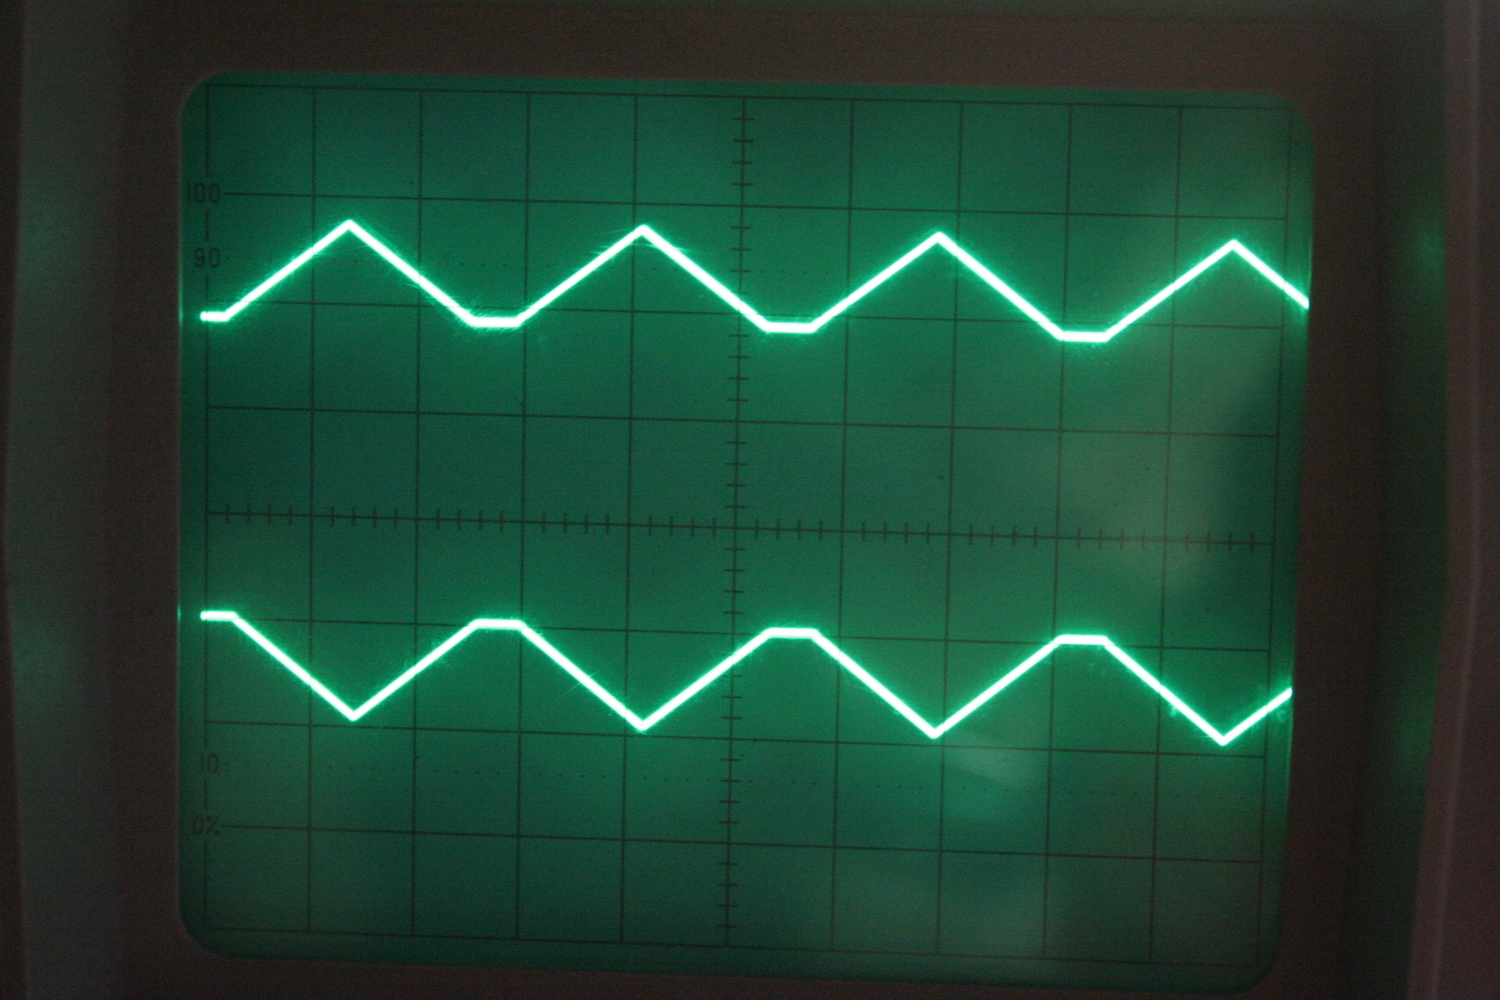
\includegraphics[width=\linewidth]{Fotos/IMG_0776-1500.jpg}
	\end{minipage}
	\caption{%
		Rechteck, Frequenz \SI{1}{\kilo\hertz},
		externe Triggerung
	}
	\label{fig:0776}
\end{figure}

\begin{figure}
	\centering
	\begin{minipage}{.45\linewidth}
	\end{minipage}
	\hfill
	\begin{minipage}{.45\linewidth}
	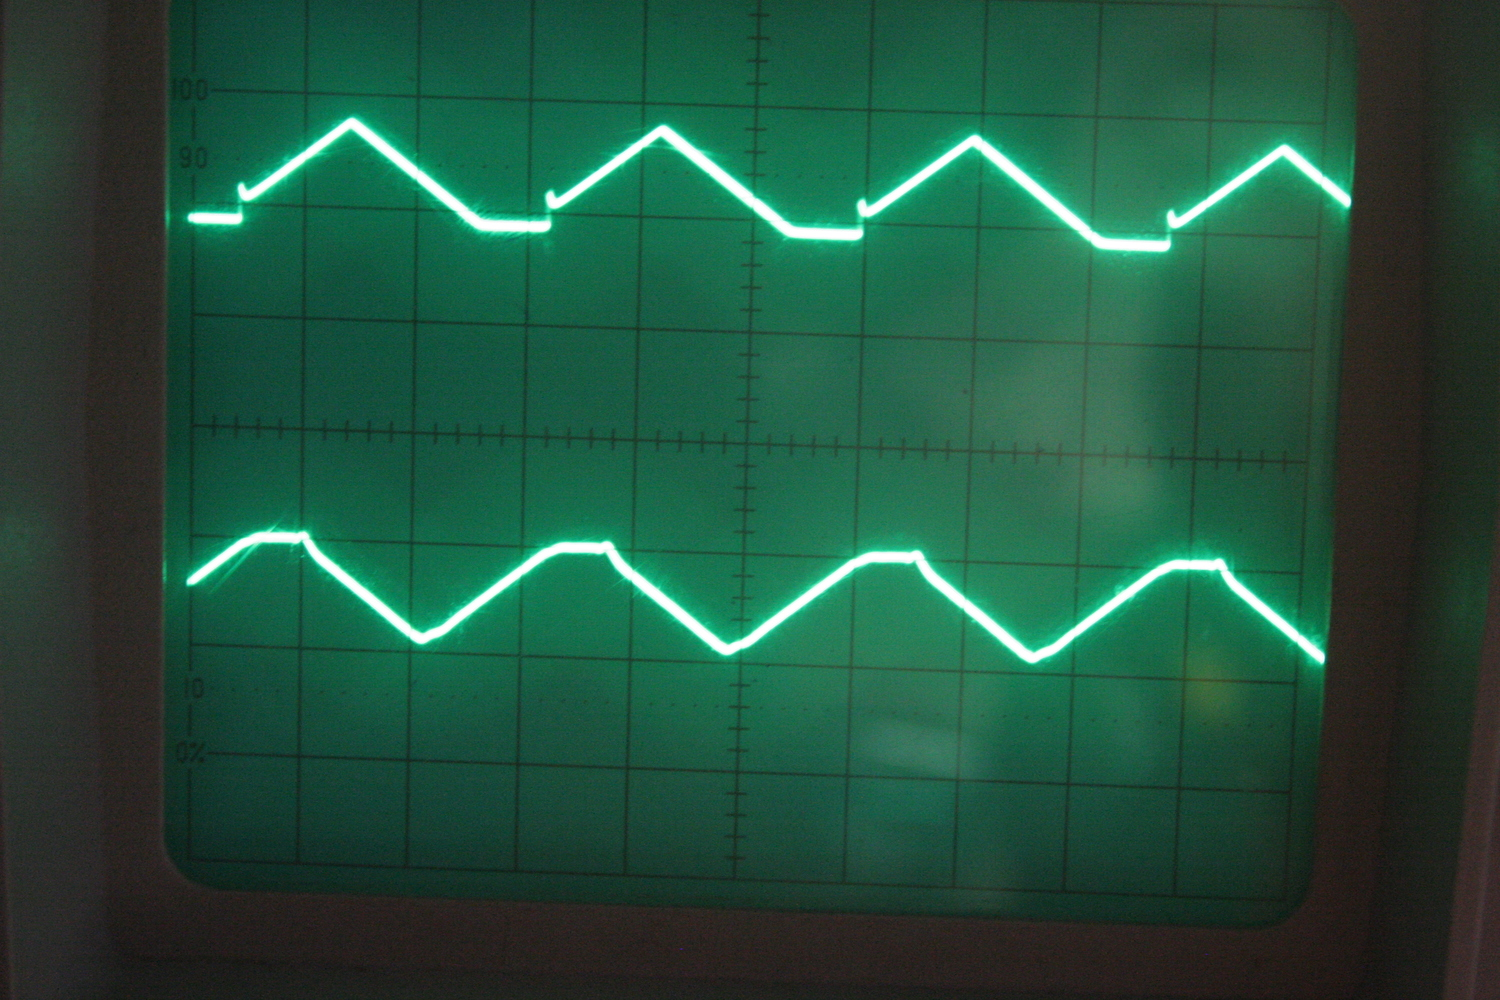
\includegraphics[width=\linewidth]{Fotos/IMG_0777-1500.jpg}
	\end{minipage}
	\caption{%
		Rechteck, Frequenz \SI{10}{\kilo\hertz},
		externe Triggerung
	}
	\label{fig:0777}
\end{figure}

\begin{figure}
	\centering
	\begin{minipage}{.45\linewidth}
	\end{minipage}
	\hfill
	\begin{minipage}{.45\linewidth}
	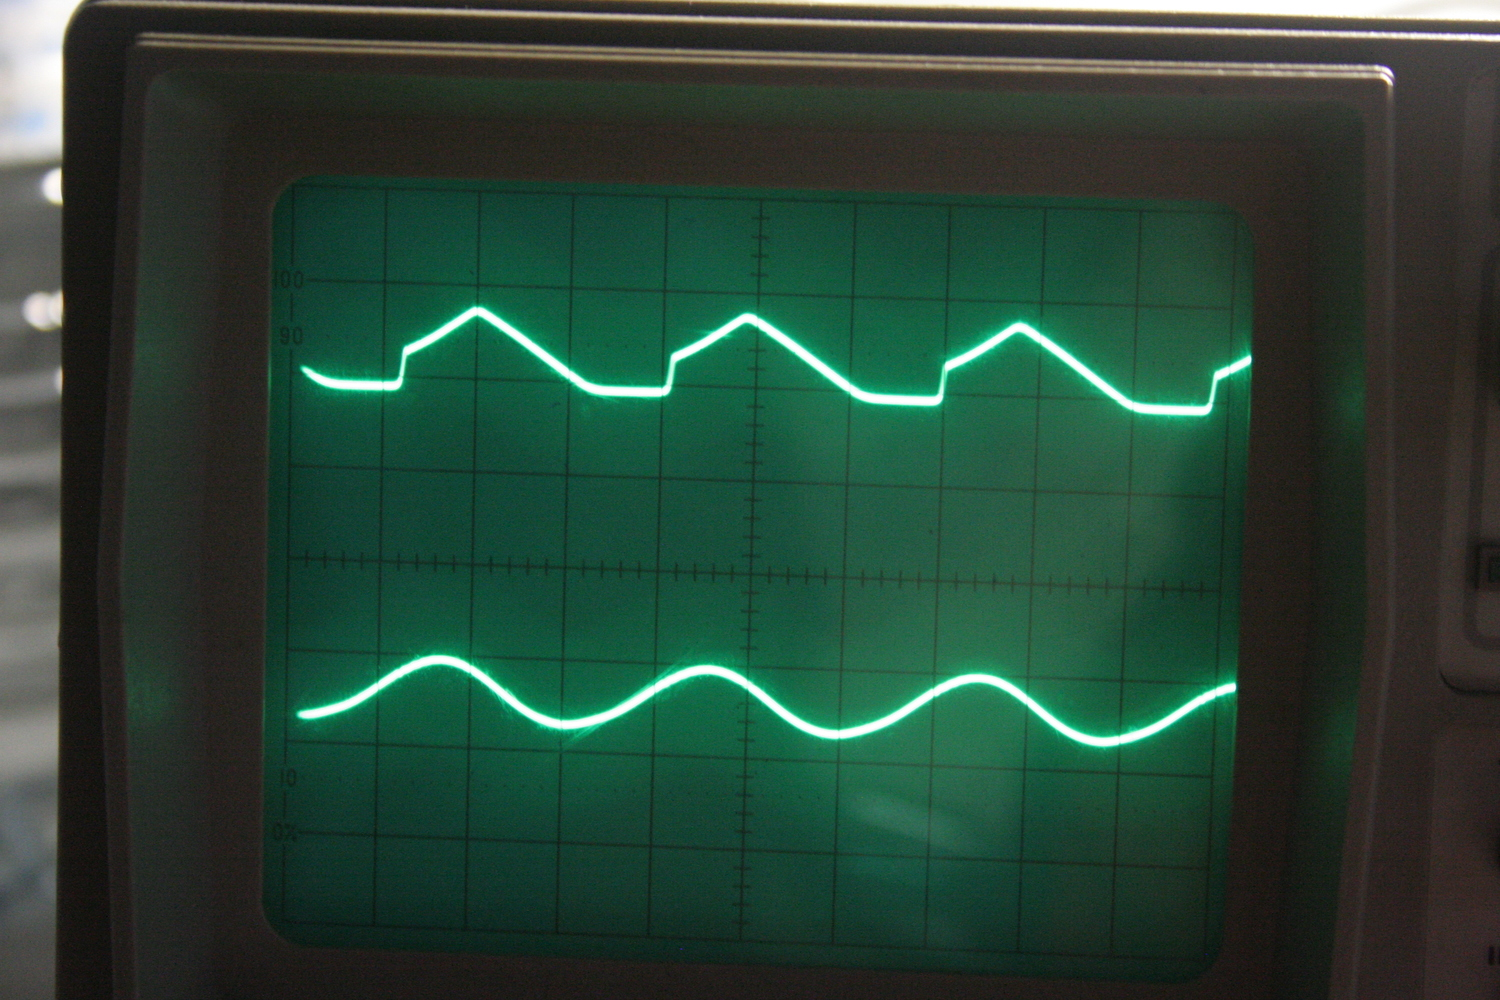
\includegraphics[width=\linewidth]{Fotos/IMG_0778-1500.jpg}
	\end{minipage}
	\caption{%
		Rechteck, Frequenz \SI{100}{\kilo\hertz},
		externe Triggerung
	}
	\label{fig:0778}
\end{figure}

\subsubsection{Teil b}

\begin{figure}
	\centering
	\begin{minipage}{.45\linewidth}
	\end{minipage}
	\hfill
	\begin{minipage}{.45\linewidth}
	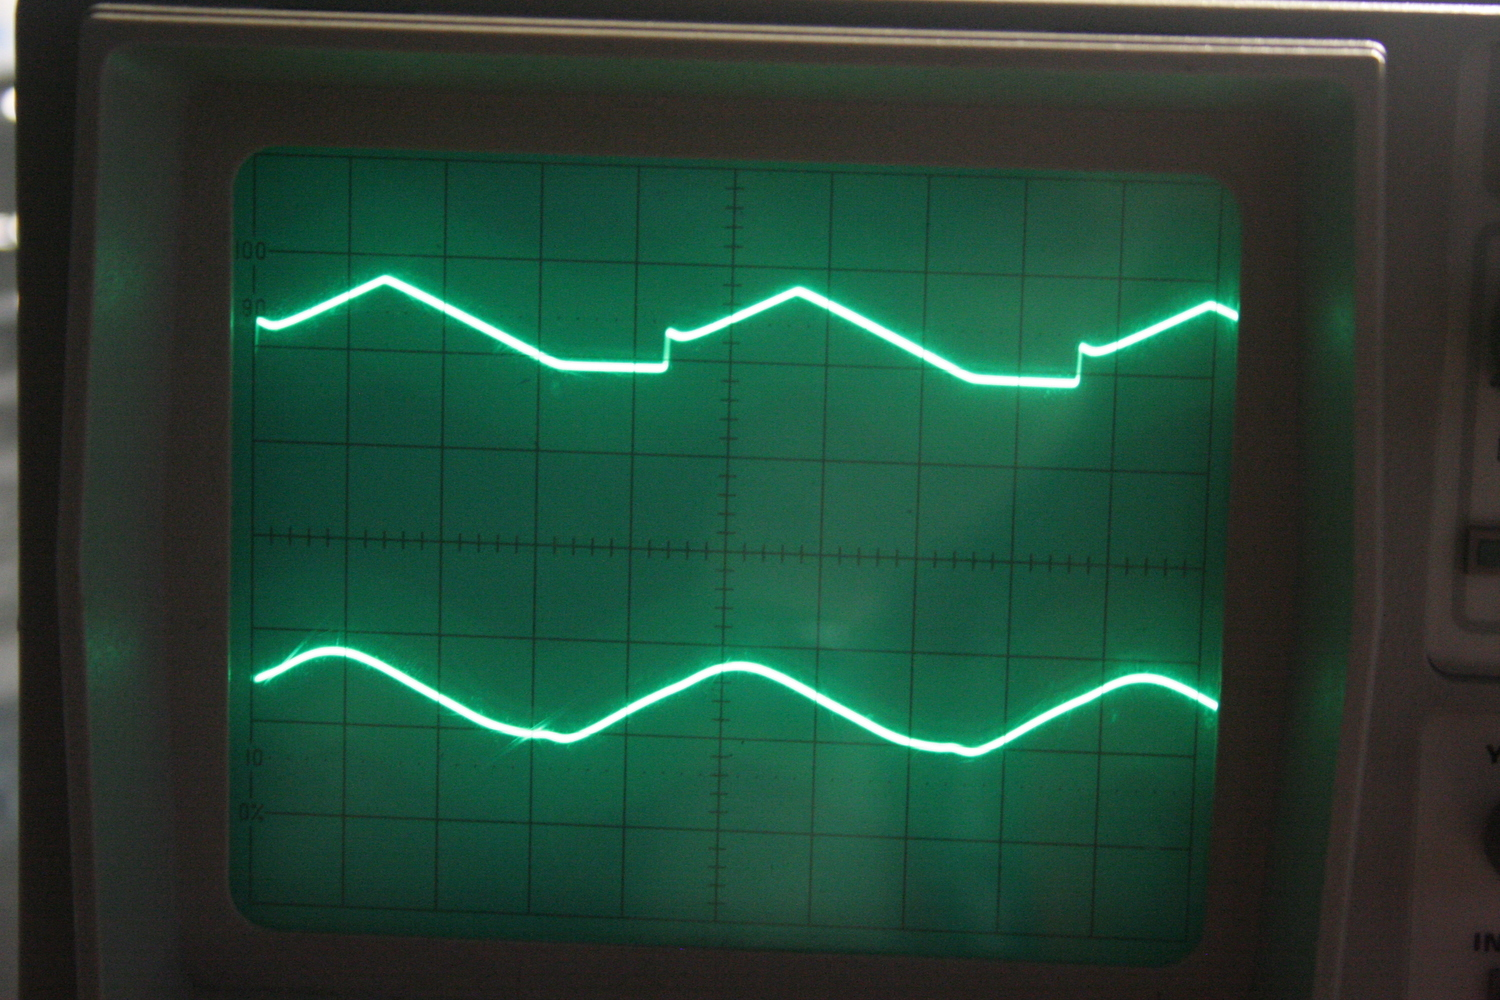
\includegraphics[width=\linewidth]{Fotos/IMG_0779-1500.jpg}
	\end{minipage}
	\caption{%
		Rechteck, Frequenz \SI{500}{\kilo\hertz},
		externe Triggerung
	}
	\label{fig:0779}
\end{figure}

%%%%%%%%%%%%%%%%%%%%%%%%%%%%%%%%%%%%%%%%%%%%%%%%%%%%%%%%%%%%%%%%%%%%%%%%%%%%%%%
%                                 Auswertung                                  %
%%%%%%%%%%%%%%%%%%%%%%%%%%%%%%%%%%%%%%%%%%%%%%%%%%%%%%%%%%%%%%%%%%%%%%%%%%%%%%%

\section{Auswertung}

\subsection{Versuchsaufgabe 3: Leitungsabschluss, Verzögerungszeit}

\subsubsection{Teil d}

%%%%%%%%%%%%%%%%%%%%%%%%%%%%%%%%%%%%%%%%%%%%%%%%%%%%%%%%%%%%%%%%%%%%%%%%%%%%%%%
%                                  Ergebnis                                   %
%%%%%%%%%%%%%%%%%%%%%%%%%%%%%%%%%%%%%%%%%%%%%%%%%%%%%%%%%%%%%%%%%%%%%%%%%%%%%%%

\section{Ergebnis}

\IfFileExists{\bibliographyfile}{
	\bibliography{\bibliographyfile}
}{}

\end{document}

% vim: spell spelllang=de
